% Created by tikzDevice version 0.6.2-92-0ad2792 on 2013-03-31 12:14:26
% !TEX encoding = UTF-8 Unicode
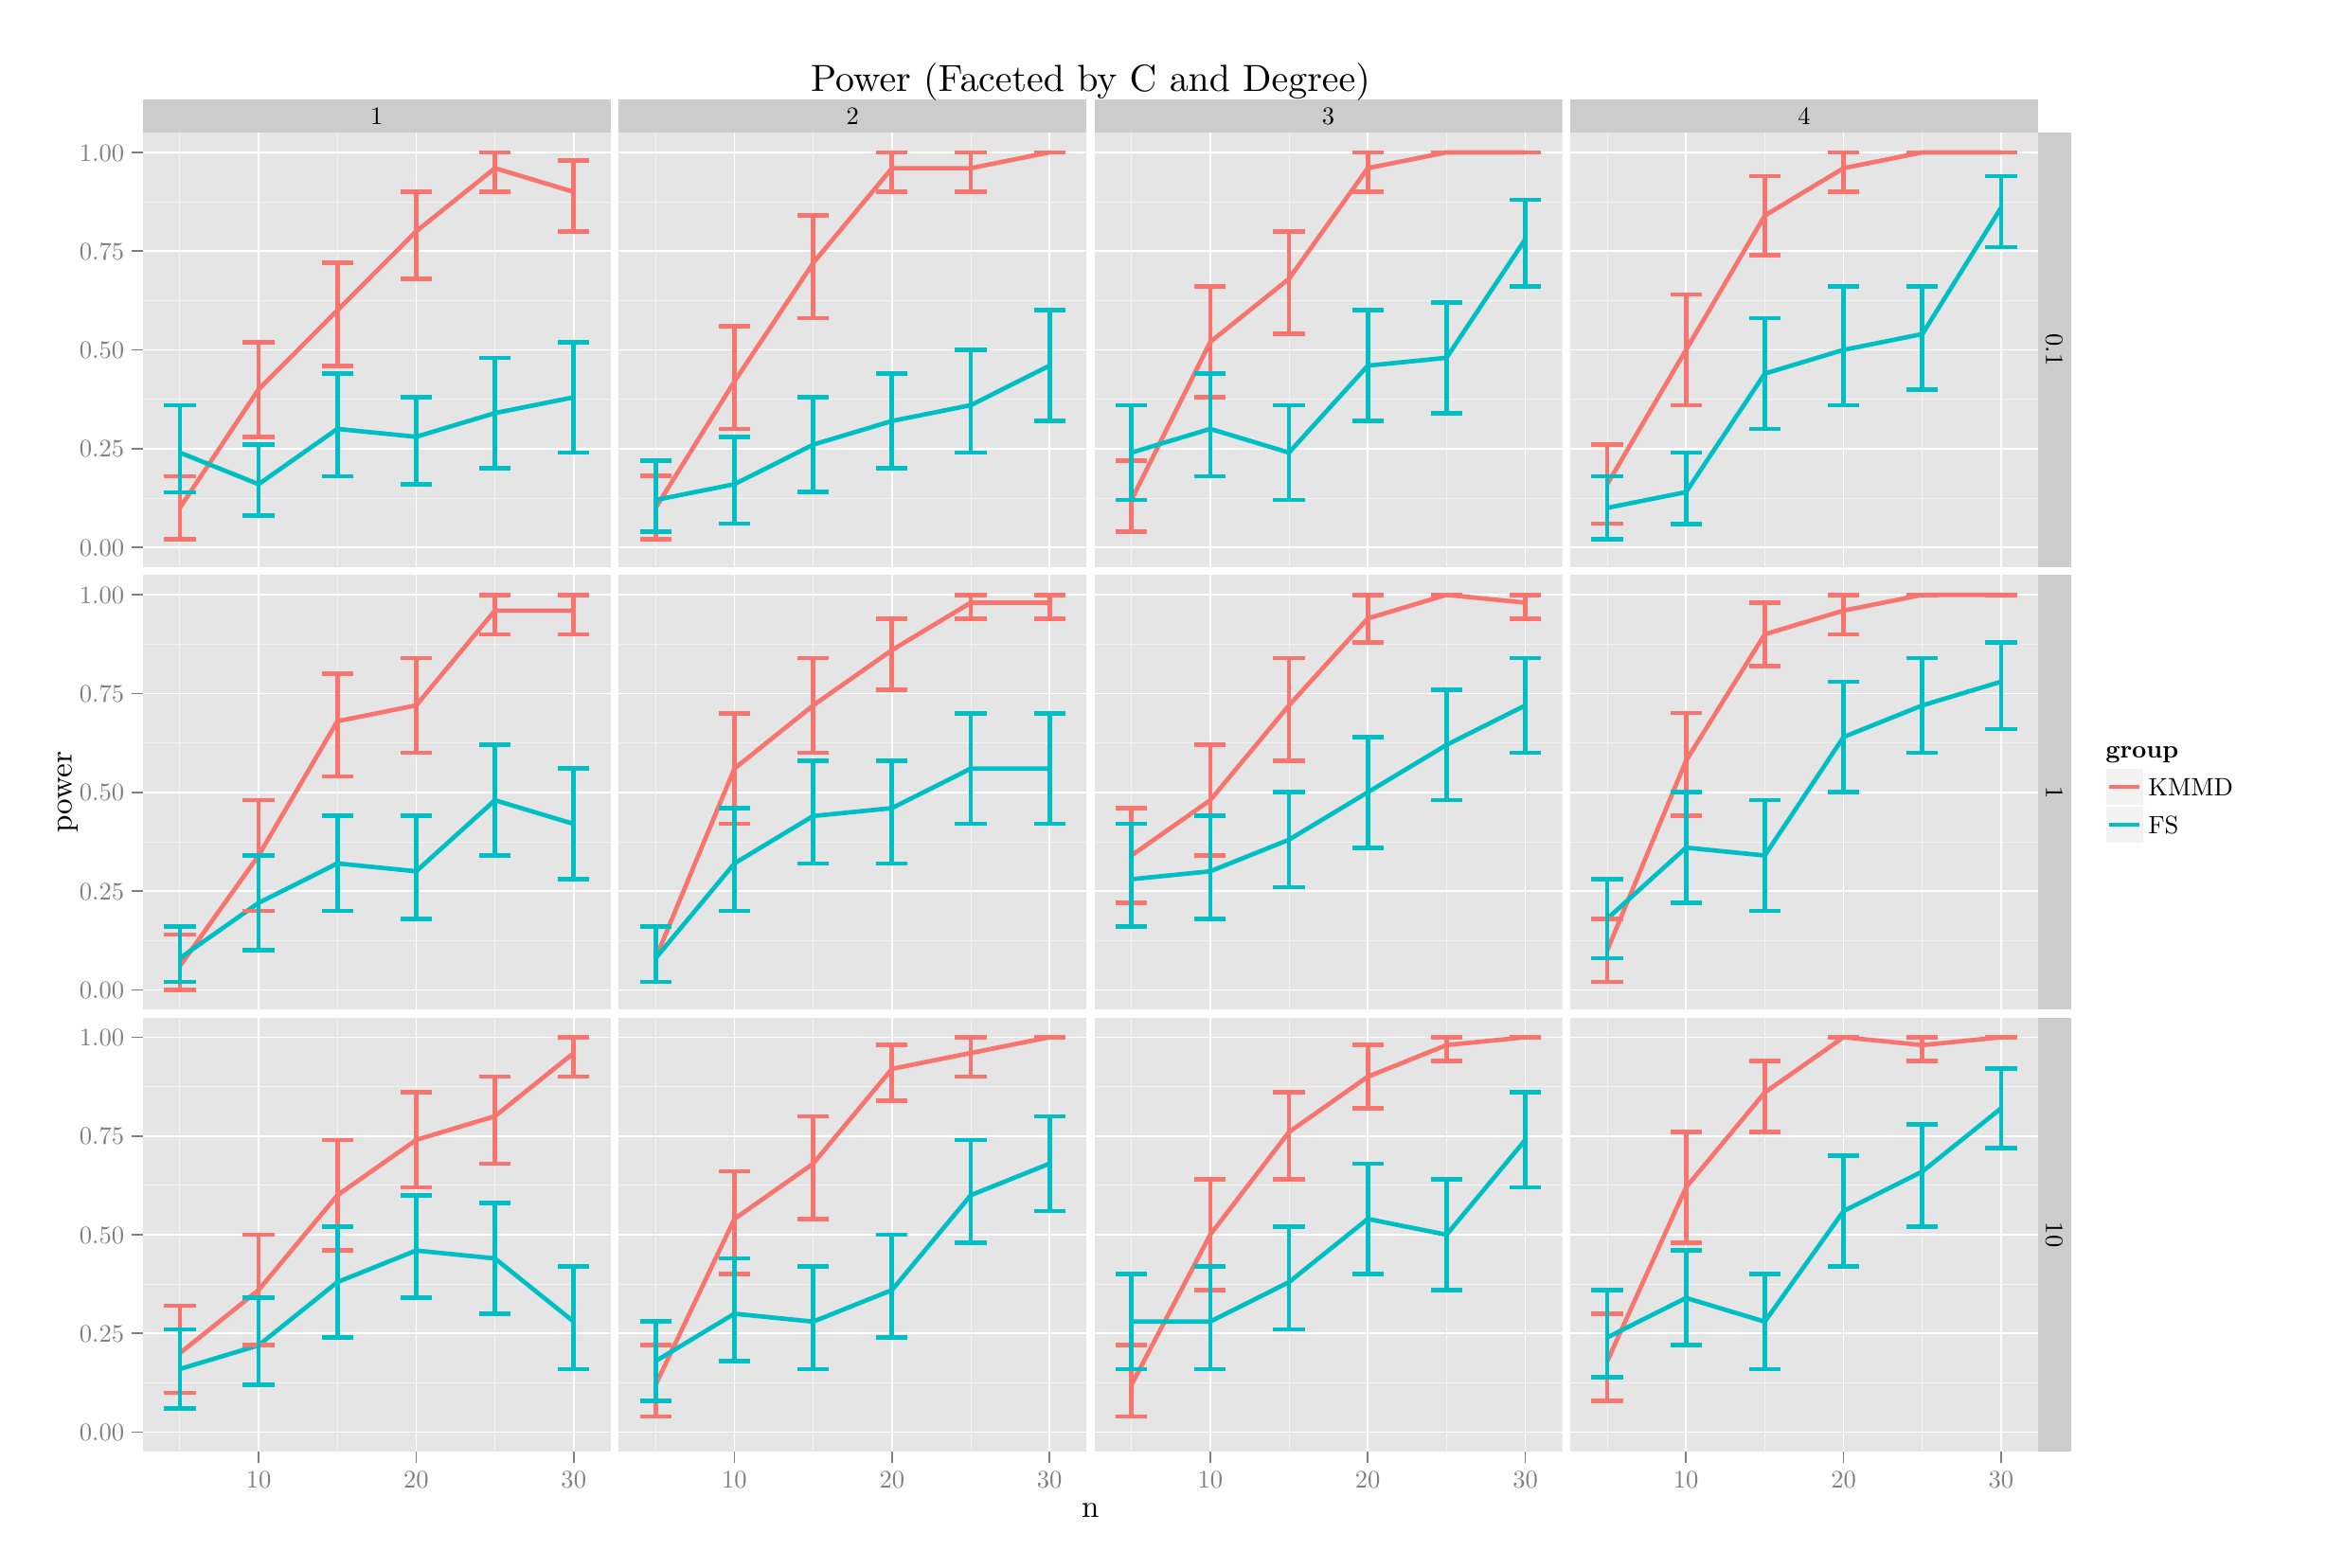
\begin{tikzpicture}[x=1pt,y=1pt]
\definecolor[named]{fillColor}{rgb}{1.00,1.00,1.00}
\path[use as bounding box,fill=fillColor,fill opacity=0.00] (0,0) rectangle (867.24,578.16);
\begin{scope}
\path[clip] (  0.00,  0.00) rectangle (867.24,578.16);
\definecolor[named]{drawColor}{rgb}{1.00,1.00,1.00}
\definecolor[named]{fillColor}{rgb}{1.00,1.00,1.00}

\path[draw=drawColor,line width= 0.6pt,line join=round,line cap=round,fill=fillColor] (  0.00, -0.00) rectangle (867.24,578.16);
\end{scope}
\begin{scope}
\path[clip] ( 44.49,537.54) rectangle (223.01,550.17);
\definecolor[named]{fillColor}{rgb}{0.80,0.80,0.80}

\path[fill=fillColor] ( 44.49,537.54) rectangle (223.01,550.17);
\definecolor[named]{drawColor}{rgb}{0.00,0.00,0.00}

\node[text=drawColor,anchor=base,inner sep=0pt, outer sep=0pt, scale=  0.96] at (133.75,540.55) {1};
\end{scope}
\begin{scope}
\path[clip] (226.03,537.54) rectangle (404.56,550.17);
\definecolor[named]{fillColor}{rgb}{0.80,0.80,0.80}

\path[fill=fillColor] (226.03,537.54) rectangle (404.56,550.17);
\definecolor[named]{drawColor}{rgb}{0.00,0.00,0.00}

\node[text=drawColor,anchor=base,inner sep=0pt, outer sep=0pt, scale=  0.96] at (315.29,540.55) {2};
\end{scope}
\begin{scope}
\path[clip] (407.57,537.54) rectangle (586.10,550.17);
\definecolor[named]{fillColor}{rgb}{0.80,0.80,0.80}

\path[fill=fillColor] (407.57,537.54) rectangle (586.10,550.17);
\definecolor[named]{drawColor}{rgb}{0.00,0.00,0.00}

\node[text=drawColor,anchor=base,inner sep=0pt, outer sep=0pt, scale=  0.96] at (496.83,540.55) {3};
\end{scope}
\begin{scope}
\path[clip] (589.11,537.54) rectangle (767.64,550.17);
\definecolor[named]{fillColor}{rgb}{0.80,0.80,0.80}

\path[fill=fillColor] (589.11,537.54) rectangle (767.64,550.17);
\definecolor[named]{drawColor}{rgb}{0.00,0.00,0.00}

\node[text=drawColor,anchor=base,inner sep=0pt, outer sep=0pt, scale=  0.96] at (678.37,540.55) {4};
\end{scope}
\begin{scope}
\path[clip] ( 44.49,371.71) rectangle (223.01,537.54);
\definecolor[named]{fillColor}{rgb}{0.90,0.90,0.90}

\path[fill=fillColor] ( 44.49,371.71) rectangle (223.01,537.54);
\definecolor[named]{drawColor}{rgb}{0.95,0.95,0.95}

\path[draw=drawColor,line width= 0.3pt,line join=round] ( 44.49,398.09) --
	(223.01,398.09);

\path[draw=drawColor,line width= 0.3pt,line join=round] ( 44.49,435.78) --
	(223.01,435.78);

\path[draw=drawColor,line width= 0.3pt,line join=round] ( 44.49,473.47) --
	(223.01,473.47);

\path[draw=drawColor,line width= 0.3pt,line join=round] ( 44.49,511.16) --
	(223.01,511.16);

\path[draw=drawColor,line width= 0.3pt,line join=round] ( 58.61,371.71) --
	( 58.61,537.54);

\path[draw=drawColor,line width= 0.3pt,line join=round] (118.72,371.71) --
	(118.72,537.54);

\path[draw=drawColor,line width= 0.3pt,line join=round] (178.83,371.71) --
	(178.83,537.54);
\definecolor[named]{drawColor}{rgb}{1.00,1.00,1.00}

\path[draw=drawColor,line width= 0.6pt,line join=round] ( 44.49,379.25) --
	(223.01,379.25);

\path[draw=drawColor,line width= 0.6pt,line join=round] ( 44.49,416.94) --
	(223.01,416.94);

\path[draw=drawColor,line width= 0.6pt,line join=round] ( 44.49,454.63) --
	(223.01,454.63);

\path[draw=drawColor,line width= 0.6pt,line join=round] ( 44.49,492.31) --
	(223.01,492.31);

\path[draw=drawColor,line width= 0.6pt,line join=round] ( 44.49,530.00) --
	(223.01,530.00);

\path[draw=drawColor,line width= 0.6pt,line join=round] ( 88.67,371.71) --
	( 88.67,537.54);

\path[draw=drawColor,line width= 0.6pt,line join=round] (148.78,371.71) --
	(148.78,537.54);

\path[draw=drawColor,line width= 0.6pt,line join=round] (208.89,371.71) --
	(208.89,537.54);
\definecolor[named]{drawColor}{rgb}{0.97,0.46,0.43}

\path[draw=drawColor,line width= 1.7pt,line join=round] ( 58.61,394.33) --
	( 88.67,439.55) --
	(118.72,469.70) --
	(148.78,499.85) --
	(178.83,523.97) --
	(208.89,514.93);
\definecolor[named]{drawColor}{rgb}{0.00,0.75,0.77}

\path[draw=drawColor,line width= 1.7pt,line join=round] ( 58.61,415.43) --
	( 88.67,403.37) --
	(118.72,424.48) --
	(148.78,421.46) --
	(178.83,430.51) --
	(208.89,436.54);
\definecolor[named]{drawColor}{rgb}{0.97,0.46,0.43}

\path[draw=drawColor,line width= 1.7pt,line join=round] ( 52.60,406.39) --
	( 64.62,406.39);

\path[draw=drawColor,line width= 1.7pt,line join=round] ( 58.61,406.39) --
	( 58.61,382.27);

\path[draw=drawColor,line width= 1.7pt,line join=round] ( 52.60,382.27) --
	( 64.62,382.27);

\path[draw=drawColor,line width= 1.7pt,line join=round] ( 82.66,457.64) --
	( 94.68,457.64);

\path[draw=drawColor,line width= 1.7pt,line join=round] ( 88.67,457.64) --
	( 88.67,421.39);

\path[draw=drawColor,line width= 1.7pt,line join=round] ( 82.66,421.39) --
	( 94.68,421.39);

\path[draw=drawColor,line width= 1.7pt,line join=round] (112.71,487.79) --
	(124.73,487.79);

\path[draw=drawColor,line width= 1.7pt,line join=round] (118.72,487.79) --
	(118.72,448.60);

\path[draw=drawColor,line width= 1.7pt,line join=round] (112.71,448.60) --
	(124.73,448.60);

\path[draw=drawColor,line width= 1.7pt,line join=round] (142.77,514.93) --
	(154.79,514.93);

\path[draw=drawColor,line width= 1.7pt,line join=round] (148.78,514.93) --
	(148.78,481.76);

\path[draw=drawColor,line width= 1.7pt,line join=round] (142.77,481.76) --
	(154.79,481.76);

\path[draw=drawColor,line width= 1.7pt,line join=round] (172.82,530.00) --
	(184.84,530.00);

\path[draw=drawColor,line width= 1.7pt,line join=round] (178.83,530.00) --
	(178.83,514.93);

\path[draw=drawColor,line width= 1.7pt,line join=round] (172.82,514.93) --
	(184.84,514.93);

\path[draw=drawColor,line width= 1.7pt,line join=round] (202.88,526.99) --
	(214.90,526.99);

\path[draw=drawColor,line width= 1.7pt,line join=round] (208.89,526.99) --
	(208.89,499.85);

\path[draw=drawColor,line width= 1.7pt,line join=round] (202.88,499.85) --
	(214.90,499.85);
\definecolor[named]{drawColor}{rgb}{0.00,0.75,0.77}

\path[draw=drawColor,line width= 1.7pt,line join=round] ( 52.60,433.52) --
	( 64.62,433.52);

\path[draw=drawColor,line width= 1.7pt,line join=round] ( 58.61,433.52) --
	( 58.61,400.28);

\path[draw=drawColor,line width= 1.7pt,line join=round] ( 52.60,400.28) --
	( 64.62,400.28);

\path[draw=drawColor,line width= 1.7pt,line join=round] ( 82.66,418.45) --
	( 94.68,418.45);

\path[draw=drawColor,line width= 1.7pt,line join=round] ( 88.67,418.45) --
	( 88.67,391.31);

\path[draw=drawColor,line width= 1.7pt,line join=round] ( 82.66,391.31) --
	( 94.68,391.31);

\path[draw=drawColor,line width= 1.7pt,line join=round] (112.71,445.58) --
	(124.73,445.58);

\path[draw=drawColor,line width= 1.7pt,line join=round] (118.72,445.58) --
	(118.72,406.39);

\path[draw=drawColor,line width= 1.7pt,line join=round] (112.71,406.39) --
	(124.73,406.39);

\path[draw=drawColor,line width= 1.7pt,line join=round] (142.77,436.54) --
	(154.79,436.54);

\path[draw=drawColor,line width= 1.7pt,line join=round] (148.78,436.54) --
	(148.78,403.37);

\path[draw=drawColor,line width= 1.7pt,line join=round] (142.77,403.37) --
	(154.79,403.37);

\path[draw=drawColor,line width= 1.7pt,line join=round] (172.82,451.61) --
	(184.84,451.61);

\path[draw=drawColor,line width= 1.7pt,line join=round] (178.83,451.61) --
	(178.83,409.40);

\path[draw=drawColor,line width= 1.7pt,line join=round] (172.82,409.40) --
	(184.84,409.40);

\path[draw=drawColor,line width= 1.7pt,line join=round] (202.88,457.64) --
	(214.90,457.64);

\path[draw=drawColor,line width= 1.7pt,line join=round] (208.89,457.64) --
	(208.89,415.43);

\path[draw=drawColor,line width= 1.7pt,line join=round] (202.88,415.43) --
	(214.90,415.43);
\end{scope}
\begin{scope}
\path[clip] ( 44.49,202.87) rectangle (223.01,368.70);
\definecolor[named]{fillColor}{rgb}{0.90,0.90,0.90}

\path[fill=fillColor] ( 44.49,202.87) rectangle (223.01,368.70);
\definecolor[named]{drawColor}{rgb}{0.95,0.95,0.95}

\path[draw=drawColor,line width= 0.3pt,line join=round] ( 44.49,229.26) --
	(223.01,229.26);

\path[draw=drawColor,line width= 0.3pt,line join=round] ( 44.49,266.94) --
	(223.01,266.94);

\path[draw=drawColor,line width= 0.3pt,line join=round] ( 44.49,304.63) --
	(223.01,304.63);

\path[draw=drawColor,line width= 0.3pt,line join=round] ( 44.49,342.32) --
	(223.01,342.32);

\path[draw=drawColor,line width= 0.3pt,line join=round] ( 58.61,202.87) --
	( 58.61,368.70);

\path[draw=drawColor,line width= 0.3pt,line join=round] (118.72,202.87) --
	(118.72,368.70);

\path[draw=drawColor,line width= 0.3pt,line join=round] (178.83,202.87) --
	(178.83,368.70);
\definecolor[named]{drawColor}{rgb}{1.00,1.00,1.00}

\path[draw=drawColor,line width= 0.6pt,line join=round] ( 44.49,210.41) --
	(223.01,210.41);

\path[draw=drawColor,line width= 0.6pt,line join=round] ( 44.49,248.10) --
	(223.01,248.10);

\path[draw=drawColor,line width= 0.6pt,line join=round] ( 44.49,285.79) --
	(223.01,285.79);

\path[draw=drawColor,line width= 0.6pt,line join=round] ( 44.49,323.48) --
	(223.01,323.48);

\path[draw=drawColor,line width= 0.6pt,line join=round] ( 44.49,361.16) --
	(223.01,361.16);

\path[draw=drawColor,line width= 0.6pt,line join=round] ( 88.67,202.87) --
	( 88.67,368.70);

\path[draw=drawColor,line width= 0.6pt,line join=round] (148.78,202.87) --
	(148.78,368.70);

\path[draw=drawColor,line width= 0.6pt,line join=round] (208.89,202.87) --
	(208.89,368.70);
\definecolor[named]{drawColor}{rgb}{0.97,0.46,0.43}

\path[draw=drawColor,line width= 1.7pt,line join=round] ( 58.61,219.46) --
	( 88.67,261.67) --
	(118.72,312.92) --
	(148.78,318.95) --
	(178.83,355.13) --
	(208.89,355.13);
\definecolor[named]{drawColor}{rgb}{0.00,0.75,0.77}

\path[draw=drawColor,line width= 1.7pt,line join=round] ( 58.61,222.47) --
	( 88.67,243.58) --
	(118.72,258.65) --
	(148.78,255.64) --
	(178.83,282.77) --
	(208.89,273.73);
\definecolor[named]{drawColor}{rgb}{0.97,0.46,0.43}

\path[draw=drawColor,line width= 1.7pt,line join=round] ( 52.60,231.52) --
	( 64.62,231.52);

\path[draw=drawColor,line width= 1.7pt,line join=round] ( 58.61,231.52) --
	( 58.61,210.41);

\path[draw=drawColor,line width= 1.7pt,line join=round] ( 52.60,210.41) --
	( 64.62,210.41);

\path[draw=drawColor,line width= 1.7pt,line join=round] ( 82.66,282.77) --
	( 94.68,282.77);

\path[draw=drawColor,line width= 1.7pt,line join=round] ( 88.67,282.77) --
	( 88.67,240.56);

\path[draw=drawColor,line width= 1.7pt,line join=round] ( 82.66,240.56) --
	( 94.68,240.56);

\path[draw=drawColor,line width= 1.7pt,line join=round] (112.71,331.01) --
	(124.73,331.01);

\path[draw=drawColor,line width= 1.7pt,line join=round] (118.72,331.01) --
	(118.72,291.82);

\path[draw=drawColor,line width= 1.7pt,line join=round] (112.71,291.82) --
	(124.73,291.82);

\path[draw=drawColor,line width= 1.7pt,line join=round] (142.77,337.04) --
	(154.79,337.04);

\path[draw=drawColor,line width= 1.7pt,line join=round] (148.78,337.04) --
	(148.78,300.86);

\path[draw=drawColor,line width= 1.7pt,line join=round] (142.77,300.86) --
	(154.79,300.86);

\path[draw=drawColor,line width= 1.7pt,line join=round] (172.82,361.16) --
	(184.84,361.16);

\path[draw=drawColor,line width= 1.7pt,line join=round] (178.83,361.16) --
	(178.83,346.09);

\path[draw=drawColor,line width= 1.7pt,line join=round] (172.82,346.09) --
	(184.84,346.09);

\path[draw=drawColor,line width= 1.7pt,line join=round] (202.88,361.16) --
	(214.90,361.16);

\path[draw=drawColor,line width= 1.7pt,line join=round] (208.89,361.16) --
	(208.89,346.09);

\path[draw=drawColor,line width= 1.7pt,line join=round] (202.88,346.09) --
	(214.90,346.09);
\definecolor[named]{drawColor}{rgb}{0.00,0.75,0.77}

\path[draw=drawColor,line width= 1.7pt,line join=round] ( 52.60,234.53) --
	( 64.62,234.53);

\path[draw=drawColor,line width= 1.7pt,line join=round] ( 58.61,234.53) --
	( 58.61,213.43);

\path[draw=drawColor,line width= 1.7pt,line join=round] ( 52.60,213.43) --
	( 64.62,213.43);

\path[draw=drawColor,line width= 1.7pt,line join=round] ( 82.66,261.67) --
	( 94.68,261.67);

\path[draw=drawColor,line width= 1.7pt,line join=round] ( 88.67,261.67) --
	( 88.67,225.49);

\path[draw=drawColor,line width= 1.7pt,line join=round] ( 82.66,225.49) --
	( 94.68,225.49);

\path[draw=drawColor,line width= 1.7pt,line join=round] (112.71,276.74) --
	(124.73,276.74);

\path[draw=drawColor,line width= 1.7pt,line join=round] (118.72,276.74) --
	(118.72,240.56);

\path[draw=drawColor,line width= 1.7pt,line join=round] (112.71,240.56) --
	(124.73,240.56);

\path[draw=drawColor,line width= 1.7pt,line join=round] (142.77,276.74) --
	(154.79,276.74);

\path[draw=drawColor,line width= 1.7pt,line join=round] (148.78,276.74) --
	(148.78,237.55);

\path[draw=drawColor,line width= 1.7pt,line join=round] (142.77,237.55) --
	(154.79,237.55);

\path[draw=drawColor,line width= 1.7pt,line join=round] (172.82,303.88) --
	(184.84,303.88);

\path[draw=drawColor,line width= 1.7pt,line join=round] (178.83,303.88) --
	(178.83,261.67);

\path[draw=drawColor,line width= 1.7pt,line join=round] (172.82,261.67) --
	(184.84,261.67);

\path[draw=drawColor,line width= 1.7pt,line join=round] (202.88,294.83) --
	(214.90,294.83);

\path[draw=drawColor,line width= 1.7pt,line join=round] (208.89,294.83) --
	(208.89,252.62);

\path[draw=drawColor,line width= 1.7pt,line join=round] (202.88,252.62) --
	(214.90,252.62);
\end{scope}
\begin{scope}
\path[clip] ( 44.49, 34.03) rectangle (223.01,199.86);
\definecolor[named]{fillColor}{rgb}{0.90,0.90,0.90}

\path[fill=fillColor] ( 44.49, 34.03) rectangle (223.01,199.86);
\definecolor[named]{drawColor}{rgb}{0.95,0.95,0.95}

\path[draw=drawColor,line width= 0.3pt,line join=round] ( 44.49, 60.42) --
	(223.01, 60.42);

\path[draw=drawColor,line width= 0.3pt,line join=round] ( 44.49, 98.10) --
	(223.01, 98.10);

\path[draw=drawColor,line width= 0.3pt,line join=round] ( 44.49,135.79) --
	(223.01,135.79);

\path[draw=drawColor,line width= 0.3pt,line join=round] ( 44.49,173.48) --
	(223.01,173.48);

\path[draw=drawColor,line width= 0.3pt,line join=round] ( 58.61, 34.03) --
	( 58.61,199.86);

\path[draw=drawColor,line width= 0.3pt,line join=round] (118.72, 34.03) --
	(118.72,199.86);

\path[draw=drawColor,line width= 0.3pt,line join=round] (178.83, 34.03) --
	(178.83,199.86);
\definecolor[named]{drawColor}{rgb}{1.00,1.00,1.00}

\path[draw=drawColor,line width= 0.6pt,line join=round] ( 44.49, 41.57) --
	(223.01, 41.57);

\path[draw=drawColor,line width= 0.6pt,line join=round] ( 44.49, 79.26) --
	(223.01, 79.26);

\path[draw=drawColor,line width= 0.6pt,line join=round] ( 44.49,116.95) --
	(223.01,116.95);

\path[draw=drawColor,line width= 0.6pt,line join=round] ( 44.49,154.64) --
	(223.01,154.64);

\path[draw=drawColor,line width= 0.6pt,line join=round] ( 44.49,192.32) --
	(223.01,192.32);

\path[draw=drawColor,line width= 0.6pt,line join=round] ( 88.67, 34.03) --
	( 88.67,199.86);

\path[draw=drawColor,line width= 0.6pt,line join=round] (148.78, 34.03) --
	(148.78,199.86);

\path[draw=drawColor,line width= 0.6pt,line join=round] (208.89, 34.03) --
	(208.89,199.86);
\definecolor[named]{drawColor}{rgb}{0.97,0.46,0.43}

\path[draw=drawColor,line width= 1.7pt,line join=round] ( 58.61, 71.72) --
	( 88.67, 95.84) --
	(118.72,132.02) --
	(148.78,153.13) --
	(178.83,162.17) --
	(208.89,186.29);
\definecolor[named]{drawColor}{rgb}{0.00,0.75,0.77}

\path[draw=drawColor,line width= 1.7pt,line join=round] ( 58.61, 65.69) --
	( 88.67, 74.74) --
	(118.72, 98.86) --
	(148.78,110.92) --
	(178.83,107.90) --
	(208.89, 83.78);
\definecolor[named]{drawColor}{rgb}{0.97,0.46,0.43}

\path[draw=drawColor,line width= 1.7pt,line join=round] ( 52.60, 89.81) --
	( 64.62, 89.81);

\path[draw=drawColor,line width= 1.7pt,line join=round] ( 58.61, 89.81) --
	( 58.61, 56.65);

\path[draw=drawColor,line width= 1.7pt,line join=round] ( 52.60, 56.65) --
	( 64.62, 56.65);

\path[draw=drawColor,line width= 1.7pt,line join=round] ( 82.66,116.95) --
	( 94.68,116.95);

\path[draw=drawColor,line width= 1.7pt,line join=round] ( 88.67,116.95) --
	( 88.67, 74.74);

\path[draw=drawColor,line width= 1.7pt,line join=round] ( 82.66, 74.74) --
	( 94.68, 74.74);

\path[draw=drawColor,line width= 1.7pt,line join=round] (112.71,153.13) --
	(124.73,153.13);

\path[draw=drawColor,line width= 1.7pt,line join=round] (118.72,153.13) --
	(118.72,110.92);

\path[draw=drawColor,line width= 1.7pt,line join=round] (112.71,110.92) --
	(124.73,110.92);

\path[draw=drawColor,line width= 1.7pt,line join=round] (142.77,171.22) --
	(154.79,171.22);

\path[draw=drawColor,line width= 1.7pt,line join=round] (148.78,171.22) --
	(148.78,135.04);

\path[draw=drawColor,line width= 1.7pt,line join=round] (142.77,135.04) --
	(154.79,135.04);

\path[draw=drawColor,line width= 1.7pt,line join=round] (172.82,177.25) --
	(184.84,177.25);

\path[draw=drawColor,line width= 1.7pt,line join=round] (178.83,177.25) --
	(178.83,144.08);

\path[draw=drawColor,line width= 1.7pt,line join=round] (172.82,144.08) --
	(184.84,144.08);

\path[draw=drawColor,line width= 1.7pt,line join=round] (202.88,192.32) --
	(214.90,192.32);

\path[draw=drawColor,line width= 1.7pt,line join=round] (208.89,192.32) --
	(208.89,177.25);

\path[draw=drawColor,line width= 1.7pt,line join=round] (202.88,177.25) --
	(214.90,177.25);
\definecolor[named]{drawColor}{rgb}{0.00,0.75,0.77}

\path[draw=drawColor,line width= 1.7pt,line join=round] ( 52.60, 80.77) --
	( 64.62, 80.77);

\path[draw=drawColor,line width= 1.7pt,line join=round] ( 58.61, 80.77) --
	( 58.61, 50.62);

\path[draw=drawColor,line width= 1.7pt,line join=round] ( 52.60, 50.62) --
	( 64.62, 50.62);

\path[draw=drawColor,line width= 1.7pt,line join=round] ( 82.66, 92.83) --
	( 94.68, 92.83);

\path[draw=drawColor,line width= 1.7pt,line join=round] ( 88.67, 92.83) --
	( 88.67, 59.66);

\path[draw=drawColor,line width= 1.7pt,line join=round] ( 82.66, 59.66) --
	( 94.68, 59.66);

\path[draw=drawColor,line width= 1.7pt,line join=round] (112.71,119.96) --
	(124.73,119.96);

\path[draw=drawColor,line width= 1.7pt,line join=round] (118.72,119.96) --
	(118.72, 77.75);

\path[draw=drawColor,line width= 1.7pt,line join=round] (112.71, 77.75) --
	(124.73, 77.75);

\path[draw=drawColor,line width= 1.7pt,line join=round] (142.77,132.02) --
	(154.79,132.02);

\path[draw=drawColor,line width= 1.7pt,line join=round] (148.78,132.02) --
	(148.78, 92.83);

\path[draw=drawColor,line width= 1.7pt,line join=round] (142.77, 92.83) --
	(154.79, 92.83);

\path[draw=drawColor,line width= 1.7pt,line join=round] (172.82,129.01) --
	(184.84,129.01);

\path[draw=drawColor,line width= 1.7pt,line join=round] (178.83,129.01) --
	(178.83, 86.80);

\path[draw=drawColor,line width= 1.7pt,line join=round] (172.82, 86.80) --
	(184.84, 86.80);

\path[draw=drawColor,line width= 1.7pt,line join=round] (202.88,104.89) --
	(214.90,104.89);

\path[draw=drawColor,line width= 1.7pt,line join=round] (208.89,104.89) --
	(208.89, 65.69);

\path[draw=drawColor,line width= 1.7pt,line join=round] (202.88, 65.69) --
	(214.90, 65.69);
\end{scope}
\begin{scope}
\path[clip] (226.03,371.71) rectangle (404.56,537.54);
\definecolor[named]{fillColor}{rgb}{0.90,0.90,0.90}

\path[fill=fillColor] (226.03,371.71) rectangle (404.56,537.54);
\definecolor[named]{drawColor}{rgb}{0.95,0.95,0.95}

\path[draw=drawColor,line width= 0.3pt,line join=round] (226.03,398.09) --
	(404.56,398.09);

\path[draw=drawColor,line width= 0.3pt,line join=round] (226.03,435.78) --
	(404.56,435.78);

\path[draw=drawColor,line width= 0.3pt,line join=round] (226.03,473.47) --
	(404.56,473.47);

\path[draw=drawColor,line width= 0.3pt,line join=round] (226.03,511.16) --
	(404.56,511.16);

\path[draw=drawColor,line width= 0.3pt,line join=round] (240.15,371.71) --
	(240.15,537.54);

\path[draw=drawColor,line width= 0.3pt,line join=round] (300.26,371.71) --
	(300.26,537.54);

\path[draw=drawColor,line width= 0.3pt,line join=round] (360.37,371.71) --
	(360.37,537.54);
\definecolor[named]{drawColor}{rgb}{1.00,1.00,1.00}

\path[draw=drawColor,line width= 0.6pt,line join=round] (226.03,379.25) --
	(404.56,379.25);

\path[draw=drawColor,line width= 0.6pt,line join=round] (226.03,416.94) --
	(404.56,416.94);

\path[draw=drawColor,line width= 0.6pt,line join=round] (226.03,454.63) --
	(404.56,454.63);

\path[draw=drawColor,line width= 0.6pt,line join=round] (226.03,492.31) --
	(404.56,492.31);

\path[draw=drawColor,line width= 0.6pt,line join=round] (226.03,530.00) --
	(404.56,530.00);

\path[draw=drawColor,line width= 0.6pt,line join=round] (270.21,371.71) --
	(270.21,537.54);

\path[draw=drawColor,line width= 0.6pt,line join=round] (330.32,371.71) --
	(330.32,537.54);

\path[draw=drawColor,line width= 0.6pt,line join=round] (390.43,371.71) --
	(390.43,537.54);
\definecolor[named]{drawColor}{rgb}{0.97,0.46,0.43}

\path[draw=drawColor,line width= 1.7pt,line join=round] (240.15,394.33) --
	(270.21,442.57) --
	(300.26,487.79) --
	(330.32,523.97) --
	(360.37,523.97) --
	(390.43,530.00);
\definecolor[named]{drawColor}{rgb}{0.00,0.75,0.77}

\path[draw=drawColor,line width= 1.7pt,line join=round] (240.15,397.34) --
	(270.21,403.37) --
	(300.26,418.45) --
	(330.32,427.49) --
	(360.37,433.52) --
	(390.43,448.60);
\definecolor[named]{drawColor}{rgb}{0.97,0.46,0.43}

\path[draw=drawColor,line width= 1.7pt,line join=round] (234.14,406.46) --
	(246.16,406.46);

\path[draw=drawColor,line width= 1.7pt,line join=round] (240.15,406.46) --
	(240.15,382.27);

\path[draw=drawColor,line width= 1.7pt,line join=round] (234.14,382.27) --
	(246.16,382.27);

\path[draw=drawColor,line width= 1.7pt,line join=round] (264.20,463.67) --
	(276.22,463.67);

\path[draw=drawColor,line width= 1.7pt,line join=round] (270.21,463.67) --
	(270.21,424.48);

\path[draw=drawColor,line width= 1.7pt,line join=round] (264.20,424.48) --
	(276.22,424.48);

\path[draw=drawColor,line width= 1.7pt,line join=round] (294.25,505.88) --
	(306.27,505.88);

\path[draw=drawColor,line width= 1.7pt,line join=round] (300.26,505.88) --
	(300.26,466.69);

\path[draw=drawColor,line width= 1.7pt,line join=round] (294.25,466.69) --
	(306.27,466.69);

\path[draw=drawColor,line width= 1.7pt,line join=round] (324.31,530.00) --
	(336.33,530.00);

\path[draw=drawColor,line width= 1.7pt,line join=round] (330.32,530.00) --
	(330.32,514.93);

\path[draw=drawColor,line width= 1.7pt,line join=round] (324.31,514.93) --
	(336.33,514.93);

\path[draw=drawColor,line width= 1.7pt,line join=round] (354.36,530.00) --
	(366.38,530.00);

\path[draw=drawColor,line width= 1.7pt,line join=round] (360.37,530.00) --
	(360.37,514.93);

\path[draw=drawColor,line width= 1.7pt,line join=round] (354.36,514.93) --
	(366.38,514.93);

\path[draw=drawColor,line width= 1.7pt,line join=round] (384.42,530.00) --
	(396.44,530.00);

\path[draw=drawColor,line width= 1.7pt,line join=round] (390.43,530.00) --
	(390.43,530.00);

\path[draw=drawColor,line width= 1.7pt,line join=round] (384.42,530.00) --
	(396.44,530.00);
\definecolor[named]{drawColor}{rgb}{0.00,0.75,0.77}

\path[draw=drawColor,line width= 1.7pt,line join=round] (234.14,412.42) --
	(246.16,412.42);

\path[draw=drawColor,line width= 1.7pt,line join=round] (240.15,412.42) --
	(240.15,385.28);

\path[draw=drawColor,line width= 1.7pt,line join=round] (234.14,385.28) --
	(246.16,385.28);

\path[draw=drawColor,line width= 1.7pt,line join=round] (264.20,421.46) --
	(276.22,421.46);

\path[draw=drawColor,line width= 1.7pt,line join=round] (270.21,421.46) --
	(270.21,388.30);

\path[draw=drawColor,line width= 1.7pt,line join=round] (264.20,388.30) --
	(276.22,388.30);

\path[draw=drawColor,line width= 1.7pt,line join=round] (294.25,436.54) --
	(306.27,436.54);

\path[draw=drawColor,line width= 1.7pt,line join=round] (300.26,436.54) --
	(300.26,400.36);

\path[draw=drawColor,line width= 1.7pt,line join=round] (294.25,400.36) --
	(306.27,400.36);

\path[draw=drawColor,line width= 1.7pt,line join=round] (324.31,445.58) --
	(336.33,445.58);

\path[draw=drawColor,line width= 1.7pt,line join=round] (330.32,445.58) --
	(330.32,409.40);

\path[draw=drawColor,line width= 1.7pt,line join=round] (324.31,409.40) --
	(336.33,409.40);

\path[draw=drawColor,line width= 1.7pt,line join=round] (354.36,454.63) --
	(366.38,454.63);

\path[draw=drawColor,line width= 1.7pt,line join=round] (360.37,454.63) --
	(360.37,415.43);

\path[draw=drawColor,line width= 1.7pt,line join=round] (354.36,415.43) --
	(366.38,415.43);

\path[draw=drawColor,line width= 1.7pt,line join=round] (384.42,469.70) --
	(396.44,469.70);

\path[draw=drawColor,line width= 1.7pt,line join=round] (390.43,469.70) --
	(390.43,427.49);

\path[draw=drawColor,line width= 1.7pt,line join=round] (384.42,427.49) --
	(396.44,427.49);
\end{scope}
\begin{scope}
\path[clip] (226.03,202.87) rectangle (404.56,368.70);
\definecolor[named]{fillColor}{rgb}{0.90,0.90,0.90}

\path[fill=fillColor] (226.03,202.87) rectangle (404.56,368.70);
\definecolor[named]{drawColor}{rgb}{0.95,0.95,0.95}

\path[draw=drawColor,line width= 0.3pt,line join=round] (226.03,229.26) --
	(404.56,229.26);

\path[draw=drawColor,line width= 0.3pt,line join=round] (226.03,266.94) --
	(404.56,266.94);

\path[draw=drawColor,line width= 0.3pt,line join=round] (226.03,304.63) --
	(404.56,304.63);

\path[draw=drawColor,line width= 0.3pt,line join=round] (226.03,342.32) --
	(404.56,342.32);

\path[draw=drawColor,line width= 0.3pt,line join=round] (240.15,202.87) --
	(240.15,368.70);

\path[draw=drawColor,line width= 0.3pt,line join=round] (300.26,202.87) --
	(300.26,368.70);

\path[draw=drawColor,line width= 0.3pt,line join=round] (360.37,202.87) --
	(360.37,368.70);
\definecolor[named]{drawColor}{rgb}{1.00,1.00,1.00}

\path[draw=drawColor,line width= 0.6pt,line join=round] (226.03,210.41) --
	(404.56,210.41);

\path[draw=drawColor,line width= 0.6pt,line join=round] (226.03,248.10) --
	(404.56,248.10);

\path[draw=drawColor,line width= 0.6pt,line join=round] (226.03,285.79) --
	(404.56,285.79);

\path[draw=drawColor,line width= 0.6pt,line join=round] (226.03,323.48) --
	(404.56,323.48);

\path[draw=drawColor,line width= 0.6pt,line join=round] (226.03,361.16) --
	(404.56,361.16);

\path[draw=drawColor,line width= 0.6pt,line join=round] (270.21,202.87) --
	(270.21,368.70);

\path[draw=drawColor,line width= 0.6pt,line join=round] (330.32,202.87) --
	(330.32,368.70);

\path[draw=drawColor,line width= 0.6pt,line join=round] (390.43,202.87) --
	(390.43,368.70);
\definecolor[named]{drawColor}{rgb}{0.97,0.46,0.43}

\path[draw=drawColor,line width= 1.7pt,line join=round] (240.15,222.47) --
	(270.21,294.83) --
	(300.26,318.95) --
	(330.32,340.06) --
	(360.37,358.15) --
	(390.43,358.15);
\definecolor[named]{drawColor}{rgb}{0.00,0.75,0.77}

\path[draw=drawColor,line width= 1.7pt,line join=round] (240.15,222.47) --
	(270.21,258.65) --
	(300.26,276.74) --
	(330.32,279.76) --
	(360.37,294.83) --
	(390.43,294.83);
\definecolor[named]{drawColor}{rgb}{0.97,0.46,0.43}

\path[draw=drawColor,line width= 1.7pt,line join=round] (234.14,234.53) --
	(246.16,234.53);

\path[draw=drawColor,line width= 1.7pt,line join=round] (240.15,234.53) --
	(240.15,213.43);

\path[draw=drawColor,line width= 1.7pt,line join=round] (234.14,213.43) --
	(246.16,213.43);

\path[draw=drawColor,line width= 1.7pt,line join=round] (264.20,315.94) --
	(276.22,315.94);

\path[draw=drawColor,line width= 1.7pt,line join=round] (270.21,315.94) --
	(270.21,273.73);

\path[draw=drawColor,line width= 1.7pt,line join=round] (264.20,273.73) --
	(276.22,273.73);

\path[draw=drawColor,line width= 1.7pt,line join=round] (294.25,337.04) --
	(306.27,337.04);

\path[draw=drawColor,line width= 1.7pt,line join=round] (300.26,337.04) --
	(300.26,300.86);

\path[draw=drawColor,line width= 1.7pt,line join=round] (294.25,300.86) --
	(306.27,300.86);

\path[draw=drawColor,line width= 1.7pt,line join=round] (324.31,352.12) --
	(336.33,352.12);

\path[draw=drawColor,line width= 1.7pt,line join=round] (330.32,352.12) --
	(330.32,324.98);

\path[draw=drawColor,line width= 1.7pt,line join=round] (324.31,324.98) --
	(336.33,324.98);

\path[draw=drawColor,line width= 1.7pt,line join=round] (354.36,361.16) --
	(366.38,361.16);

\path[draw=drawColor,line width= 1.7pt,line join=round] (360.37,361.16) --
	(360.37,352.12);

\path[draw=drawColor,line width= 1.7pt,line join=round] (354.36,352.12) --
	(366.38,352.12);

\path[draw=drawColor,line width= 1.7pt,line join=round] (384.42,361.16) --
	(396.44,361.16);

\path[draw=drawColor,line width= 1.7pt,line join=round] (390.43,361.16) --
	(390.43,352.12);

\path[draw=drawColor,line width= 1.7pt,line join=round] (384.42,352.12) --
	(396.44,352.12);
\definecolor[named]{drawColor}{rgb}{0.00,0.75,0.77}

\path[draw=drawColor,line width= 1.7pt,line join=round] (234.14,234.53) --
	(246.16,234.53);

\path[draw=drawColor,line width= 1.7pt,line join=round] (240.15,234.53) --
	(240.15,213.43);

\path[draw=drawColor,line width= 1.7pt,line join=round] (234.14,213.43) --
	(246.16,213.43);

\path[draw=drawColor,line width= 1.7pt,line join=round] (264.20,279.76) --
	(276.22,279.76);

\path[draw=drawColor,line width= 1.7pt,line join=round] (270.21,279.76) --
	(270.21,240.56);

\path[draw=drawColor,line width= 1.7pt,line join=round] (264.20,240.56) --
	(276.22,240.56);

\path[draw=drawColor,line width= 1.7pt,line join=round] (294.25,297.85) --
	(306.27,297.85);

\path[draw=drawColor,line width= 1.7pt,line join=round] (300.26,297.85) --
	(300.26,258.65);

\path[draw=drawColor,line width= 1.7pt,line join=round] (294.25,258.65) --
	(306.27,258.65);

\path[draw=drawColor,line width= 1.7pt,line join=round] (324.31,297.85) --
	(336.33,297.85);

\path[draw=drawColor,line width= 1.7pt,line join=round] (330.32,297.85) --
	(330.32,258.65);

\path[draw=drawColor,line width= 1.7pt,line join=round] (324.31,258.65) --
	(336.33,258.65);

\path[draw=drawColor,line width= 1.7pt,line join=round] (354.36,315.94) --
	(366.38,315.94);

\path[draw=drawColor,line width= 1.7pt,line join=round] (360.37,315.94) --
	(360.37,273.73);

\path[draw=drawColor,line width= 1.7pt,line join=round] (354.36,273.73) --
	(366.38,273.73);

\path[draw=drawColor,line width= 1.7pt,line join=round] (384.42,315.94) --
	(396.44,315.94);

\path[draw=drawColor,line width= 1.7pt,line join=round] (390.43,315.94) --
	(390.43,273.73);

\path[draw=drawColor,line width= 1.7pt,line join=round] (384.42,273.73) --
	(396.44,273.73);
\end{scope}
\begin{scope}
\path[clip] (226.03, 34.03) rectangle (404.56,199.86);
\definecolor[named]{fillColor}{rgb}{0.90,0.90,0.90}

\path[fill=fillColor] (226.03, 34.03) rectangle (404.56,199.86);
\definecolor[named]{drawColor}{rgb}{0.95,0.95,0.95}

\path[draw=drawColor,line width= 0.3pt,line join=round] (226.03, 60.42) --
	(404.56, 60.42);

\path[draw=drawColor,line width= 0.3pt,line join=round] (226.03, 98.10) --
	(404.56, 98.10);

\path[draw=drawColor,line width= 0.3pt,line join=round] (226.03,135.79) --
	(404.56,135.79);

\path[draw=drawColor,line width= 0.3pt,line join=round] (226.03,173.48) --
	(404.56,173.48);

\path[draw=drawColor,line width= 0.3pt,line join=round] (240.15, 34.03) --
	(240.15,199.86);

\path[draw=drawColor,line width= 0.3pt,line join=round] (300.26, 34.03) --
	(300.26,199.86);

\path[draw=drawColor,line width= 0.3pt,line join=round] (360.37, 34.03) --
	(360.37,199.86);
\definecolor[named]{drawColor}{rgb}{1.00,1.00,1.00}

\path[draw=drawColor,line width= 0.6pt,line join=round] (226.03, 41.57) --
	(404.56, 41.57);

\path[draw=drawColor,line width= 0.6pt,line join=round] (226.03, 79.26) --
	(404.56, 79.26);

\path[draw=drawColor,line width= 0.6pt,line join=round] (226.03,116.95) --
	(404.56,116.95);

\path[draw=drawColor,line width= 0.6pt,line join=round] (226.03,154.64) --
	(404.56,154.64);

\path[draw=drawColor,line width= 0.6pt,line join=round] (226.03,192.32) --
	(404.56,192.32);

\path[draw=drawColor,line width= 0.6pt,line join=round] (270.21, 34.03) --
	(270.21,199.86);

\path[draw=drawColor,line width= 0.6pt,line join=round] (330.32, 34.03) --
	(330.32,199.86);

\path[draw=drawColor,line width= 0.6pt,line join=round] (390.43, 34.03) --
	(390.43,199.86);
\definecolor[named]{drawColor}{rgb}{0.97,0.46,0.43}

\path[draw=drawColor,line width= 1.7pt,line join=round] (240.15, 59.66) --
	(270.21,122.98) --
	(300.26,144.08) --
	(330.32,180.26) --
	(360.37,186.29) --
	(390.43,192.32);
\definecolor[named]{drawColor}{rgb}{0.00,0.75,0.77}

\path[draw=drawColor,line width= 1.7pt,line join=round] (240.15, 68.71) --
	(270.21, 86.80) --
	(300.26, 83.78) --
	(330.32, 95.84) --
	(360.37,132.02) --
	(390.43,144.08);
\definecolor[named]{drawColor}{rgb}{0.97,0.46,0.43}

\path[draw=drawColor,line width= 1.7pt,line join=round] (234.14, 74.74) --
	(246.16, 74.74);

\path[draw=drawColor,line width= 1.7pt,line join=round] (240.15, 74.74) --
	(240.15, 47.60);

\path[draw=drawColor,line width= 1.7pt,line join=round] (234.14, 47.60) --
	(246.16, 47.60);

\path[draw=drawColor,line width= 1.7pt,line join=round] (264.20,141.14) --
	(276.22,141.14);

\path[draw=drawColor,line width= 1.7pt,line join=round] (270.21,141.14) --
	(270.21,101.87);

\path[draw=drawColor,line width= 1.7pt,line join=round] (264.20,101.87) --
	(276.22,101.87);

\path[draw=drawColor,line width= 1.7pt,line join=round] (294.25,162.17) --
	(306.27,162.17);

\path[draw=drawColor,line width= 1.7pt,line join=round] (300.26,162.17) --
	(300.26,122.98);

\path[draw=drawColor,line width= 1.7pt,line join=round] (294.25,122.98) --
	(306.27,122.98);

\path[draw=drawColor,line width= 1.7pt,line join=round] (324.31,189.31) --
	(336.33,189.31);

\path[draw=drawColor,line width= 1.7pt,line join=round] (330.32,189.31) --
	(330.32,168.20);

\path[draw=drawColor,line width= 1.7pt,line join=round] (324.31,168.20) --
	(336.33,168.20);

\path[draw=drawColor,line width= 1.7pt,line join=round] (354.36,192.32) --
	(366.38,192.32);

\path[draw=drawColor,line width= 1.7pt,line join=round] (360.37,192.32) --
	(360.37,177.25);

\path[draw=drawColor,line width= 1.7pt,line join=round] (354.36,177.25) --
	(366.38,177.25);

\path[draw=drawColor,line width= 1.7pt,line join=round] (384.42,192.32) --
	(396.44,192.32);

\path[draw=drawColor,line width= 1.7pt,line join=round] (390.43,192.32) --
	(390.43,192.32);

\path[draw=drawColor,line width= 1.7pt,line join=round] (384.42,192.32) --
	(396.44,192.32);
\definecolor[named]{drawColor}{rgb}{0.00,0.75,0.77}

\path[draw=drawColor,line width= 1.7pt,line join=round] (234.14, 83.78) --
	(246.16, 83.78);

\path[draw=drawColor,line width= 1.7pt,line join=round] (240.15, 83.78) --
	(240.15, 53.63);

\path[draw=drawColor,line width= 1.7pt,line join=round] (234.14, 53.63) --
	(246.16, 53.63);

\path[draw=drawColor,line width= 1.7pt,line join=round] (264.20,107.90) --
	(276.22,107.90);

\path[draw=drawColor,line width= 1.7pt,line join=round] (270.21,107.90) --
	(270.21, 68.71);

\path[draw=drawColor,line width= 1.7pt,line join=round] (264.20, 68.71) --
	(276.22, 68.71);

\path[draw=drawColor,line width= 1.7pt,line join=round] (294.25,104.89) --
	(306.27,104.89);

\path[draw=drawColor,line width= 1.7pt,line join=round] (300.26,104.89) --
	(300.26, 65.69);

\path[draw=drawColor,line width= 1.7pt,line join=round] (294.25, 65.69) --
	(306.27, 65.69);

\path[draw=drawColor,line width= 1.7pt,line join=round] (324.31,116.95) --
	(336.33,116.95);

\path[draw=drawColor,line width= 1.7pt,line join=round] (330.32,116.95) --
	(330.32, 77.75);

\path[draw=drawColor,line width= 1.7pt,line join=round] (324.31, 77.75) --
	(336.33, 77.75);

\path[draw=drawColor,line width= 1.7pt,line join=round] (354.36,153.13) --
	(366.38,153.13);

\path[draw=drawColor,line width= 1.7pt,line join=round] (360.37,153.13) --
	(360.37,113.93);

\path[draw=drawColor,line width= 1.7pt,line join=round] (354.36,113.93) --
	(366.38,113.93);

\path[draw=drawColor,line width= 1.7pt,line join=round] (384.42,162.17) --
	(396.44,162.17);

\path[draw=drawColor,line width= 1.7pt,line join=round] (390.43,162.17) --
	(390.43,125.99);

\path[draw=drawColor,line width= 1.7pt,line join=round] (384.42,125.99) --
	(396.44,125.99);
\end{scope}
\begin{scope}
\path[clip] (407.57,371.71) rectangle (586.10,537.54);
\definecolor[named]{fillColor}{rgb}{0.90,0.90,0.90}

\path[fill=fillColor] (407.57,371.71) rectangle (586.10,537.54);
\definecolor[named]{drawColor}{rgb}{0.95,0.95,0.95}

\path[draw=drawColor,line width= 0.3pt,line join=round] (407.57,398.09) --
	(586.10,398.09);

\path[draw=drawColor,line width= 0.3pt,line join=round] (407.57,435.78) --
	(586.10,435.78);

\path[draw=drawColor,line width= 0.3pt,line join=round] (407.57,473.47) --
	(586.10,473.47);

\path[draw=drawColor,line width= 0.3pt,line join=round] (407.57,511.16) --
	(586.10,511.16);

\path[draw=drawColor,line width= 0.3pt,line join=round] (421.69,371.71) --
	(421.69,537.54);

\path[draw=drawColor,line width= 0.3pt,line join=round] (481.80,371.71) --
	(481.80,537.54);

\path[draw=drawColor,line width= 0.3pt,line join=round] (541.91,371.71) --
	(541.91,537.54);
\definecolor[named]{drawColor}{rgb}{1.00,1.00,1.00}

\path[draw=drawColor,line width= 0.6pt,line join=round] (407.57,379.25) --
	(586.10,379.25);

\path[draw=drawColor,line width= 0.6pt,line join=round] (407.57,416.94) --
	(586.10,416.94);

\path[draw=drawColor,line width= 0.6pt,line join=round] (407.57,454.63) --
	(586.10,454.63);

\path[draw=drawColor,line width= 0.6pt,line join=round] (407.57,492.31) --
	(586.10,492.31);

\path[draw=drawColor,line width= 0.6pt,line join=round] (407.57,530.00) --
	(586.10,530.00);

\path[draw=drawColor,line width= 0.6pt,line join=round] (451.75,371.71) --
	(451.75,537.54);

\path[draw=drawColor,line width= 0.6pt,line join=round] (511.86,371.71) --
	(511.86,537.54);

\path[draw=drawColor,line width= 0.6pt,line join=round] (571.97,371.71) --
	(571.97,537.54);
\definecolor[named]{drawColor}{rgb}{0.97,0.46,0.43}

\path[draw=drawColor,line width= 1.7pt,line join=round] (421.69,397.34) --
	(451.75,457.64) --
	(481.80,481.76) --
	(511.86,523.97) --
	(541.91,530.00) --
	(571.97,530.00);
\definecolor[named]{drawColor}{rgb}{0.00,0.75,0.77}

\path[draw=drawColor,line width= 1.7pt,line join=round] (421.69,415.43) --
	(451.75,424.48) --
	(481.80,415.43) --
	(511.86,448.60) --
	(541.91,451.61) --
	(571.97,496.84);
\definecolor[named]{drawColor}{rgb}{0.97,0.46,0.43}

\path[draw=drawColor,line width= 1.7pt,line join=round] (415.68,412.42) --
	(427.70,412.42);

\path[draw=drawColor,line width= 1.7pt,line join=round] (421.69,412.42) --
	(421.69,385.28);

\path[draw=drawColor,line width= 1.7pt,line join=round] (415.68,385.28) --
	(427.70,385.28);

\path[draw=drawColor,line width= 1.7pt,line join=round] (445.74,478.75) --
	(457.76,478.75);

\path[draw=drawColor,line width= 1.7pt,line join=round] (451.75,478.75) --
	(451.75,436.54);

\path[draw=drawColor,line width= 1.7pt,line join=round] (445.74,436.54) --
	(457.76,436.54);

\path[draw=drawColor,line width= 1.7pt,line join=round] (475.79,499.85) --
	(487.81,499.85);

\path[draw=drawColor,line width= 1.7pt,line join=round] (481.80,499.85) --
	(481.80,460.66);

\path[draw=drawColor,line width= 1.7pt,line join=round] (475.79,460.66) --
	(487.81,460.66);

\path[draw=drawColor,line width= 1.7pt,line join=round] (505.85,530.00) --
	(517.87,530.00);

\path[draw=drawColor,line width= 1.7pt,line join=round] (511.86,530.00) --
	(511.86,514.93);

\path[draw=drawColor,line width= 1.7pt,line join=round] (505.85,514.93) --
	(517.87,514.93);

\path[draw=drawColor,line width= 1.7pt,line join=round] (535.90,530.00) --
	(547.93,530.00);

\path[draw=drawColor,line width= 1.7pt,line join=round] (541.91,530.00) --
	(541.91,530.00);

\path[draw=drawColor,line width= 1.7pt,line join=round] (535.90,530.00) --
	(547.93,530.00);

\path[draw=drawColor,line width= 1.7pt,line join=round] (565.96,530.00) --
	(577.98,530.00);

\path[draw=drawColor,line width= 1.7pt,line join=round] (571.97,530.00) --
	(571.97,530.00);

\path[draw=drawColor,line width= 1.7pt,line join=round] (565.96,530.00) --
	(577.98,530.00);
\definecolor[named]{drawColor}{rgb}{0.00,0.75,0.77}

\path[draw=drawColor,line width= 1.7pt,line join=round] (415.68,433.52) --
	(427.70,433.52);

\path[draw=drawColor,line width= 1.7pt,line join=round] (421.69,433.52) --
	(421.69,397.34);

\path[draw=drawColor,line width= 1.7pt,line join=round] (415.68,397.34) --
	(427.70,397.34);

\path[draw=drawColor,line width= 1.7pt,line join=round] (445.74,445.58) --
	(457.76,445.58);

\path[draw=drawColor,line width= 1.7pt,line join=round] (451.75,445.58) --
	(451.75,406.39);

\path[draw=drawColor,line width= 1.7pt,line join=round] (445.74,406.39) --
	(457.76,406.39);

\path[draw=drawColor,line width= 1.7pt,line join=round] (475.79,433.52) --
	(487.81,433.52);

\path[draw=drawColor,line width= 1.7pt,line join=round] (481.80,433.52) --
	(481.80,397.34);

\path[draw=drawColor,line width= 1.7pt,line join=round] (475.79,397.34) --
	(487.81,397.34);

\path[draw=drawColor,line width= 1.7pt,line join=round] (505.85,469.70) --
	(517.87,469.70);

\path[draw=drawColor,line width= 1.7pt,line join=round] (511.86,469.70) --
	(511.86,427.49);

\path[draw=drawColor,line width= 1.7pt,line join=round] (505.85,427.49) --
	(517.87,427.49);

\path[draw=drawColor,line width= 1.7pt,line join=round] (535.90,472.72) --
	(547.93,472.72);

\path[draw=drawColor,line width= 1.7pt,line join=round] (541.91,472.72) --
	(541.91,430.51);

\path[draw=drawColor,line width= 1.7pt,line join=round] (535.90,430.51) --
	(547.93,430.51);

\path[draw=drawColor,line width= 1.7pt,line join=round] (565.96,511.91) --
	(577.98,511.91);

\path[draw=drawColor,line width= 1.7pt,line join=round] (571.97,511.91) --
	(571.97,478.75);

\path[draw=drawColor,line width= 1.7pt,line join=round] (565.96,478.75) --
	(577.98,478.75);
\end{scope}
\begin{scope}
\path[clip] (407.57,202.87) rectangle (586.10,368.70);
\definecolor[named]{fillColor}{rgb}{0.90,0.90,0.90}

\path[fill=fillColor] (407.57,202.87) rectangle (586.10,368.70);
\definecolor[named]{drawColor}{rgb}{0.95,0.95,0.95}

\path[draw=drawColor,line width= 0.3pt,line join=round] (407.57,229.26) --
	(586.10,229.26);

\path[draw=drawColor,line width= 0.3pt,line join=round] (407.57,266.94) --
	(586.10,266.94);

\path[draw=drawColor,line width= 0.3pt,line join=round] (407.57,304.63) --
	(586.10,304.63);

\path[draw=drawColor,line width= 0.3pt,line join=round] (407.57,342.32) --
	(586.10,342.32);

\path[draw=drawColor,line width= 0.3pt,line join=round] (421.69,202.87) --
	(421.69,368.70);

\path[draw=drawColor,line width= 0.3pt,line join=round] (481.80,202.87) --
	(481.80,368.70);

\path[draw=drawColor,line width= 0.3pt,line join=round] (541.91,202.87) --
	(541.91,368.70);
\definecolor[named]{drawColor}{rgb}{1.00,1.00,1.00}

\path[draw=drawColor,line width= 0.6pt,line join=round] (407.57,210.41) --
	(586.10,210.41);

\path[draw=drawColor,line width= 0.6pt,line join=round] (407.57,248.10) --
	(586.10,248.10);

\path[draw=drawColor,line width= 0.6pt,line join=round] (407.57,285.79) --
	(586.10,285.79);

\path[draw=drawColor,line width= 0.6pt,line join=round] (407.57,323.48) --
	(586.10,323.48);

\path[draw=drawColor,line width= 0.6pt,line join=round] (407.57,361.16) --
	(586.10,361.16);

\path[draw=drawColor,line width= 0.6pt,line join=round] (451.75,202.87) --
	(451.75,368.70);

\path[draw=drawColor,line width= 0.6pt,line join=round] (511.86,202.87) --
	(511.86,368.70);

\path[draw=drawColor,line width= 0.6pt,line join=round] (571.97,202.87) --
	(571.97,368.70);
\definecolor[named]{drawColor}{rgb}{0.97,0.46,0.43}

\path[draw=drawColor,line width= 1.7pt,line join=round] (421.69,261.67) --
	(451.75,282.77) --
	(481.80,318.95) --
	(511.86,352.12) --
	(541.91,361.16) --
	(571.97,358.15);
\definecolor[named]{drawColor}{rgb}{0.00,0.75,0.77}

\path[draw=drawColor,line width= 1.7pt,line join=round] (421.69,252.62) --
	(451.75,255.64) --
	(481.80,267.70) --
	(511.86,285.79) --
	(541.91,303.88) --
	(571.97,318.95);
\definecolor[named]{drawColor}{rgb}{0.97,0.46,0.43}

\path[draw=drawColor,line width= 1.7pt,line join=round] (415.68,279.76) --
	(427.70,279.76);

\path[draw=drawColor,line width= 1.7pt,line join=round] (421.69,279.76) --
	(421.69,243.58);

\path[draw=drawColor,line width= 1.7pt,line join=round] (415.68,243.58) --
	(427.70,243.58);

\path[draw=drawColor,line width= 1.7pt,line join=round] (445.74,303.88) --
	(457.76,303.88);

\path[draw=drawColor,line width= 1.7pt,line join=round] (451.75,303.88) --
	(451.75,261.67);

\path[draw=drawColor,line width= 1.7pt,line join=round] (445.74,261.67) --
	(457.76,261.67);

\path[draw=drawColor,line width= 1.7pt,line join=round] (475.79,337.04) --
	(487.81,337.04);

\path[draw=drawColor,line width= 1.7pt,line join=round] (481.80,337.04) --
	(481.80,297.85);

\path[draw=drawColor,line width= 1.7pt,line join=round] (475.79,297.85) --
	(487.81,297.85);

\path[draw=drawColor,line width= 1.7pt,line join=round] (505.85,361.16) --
	(517.87,361.16);

\path[draw=drawColor,line width= 1.7pt,line join=round] (511.86,361.16) --
	(511.86,343.07);

\path[draw=drawColor,line width= 1.7pt,line join=round] (505.85,343.07) --
	(517.87,343.07);

\path[draw=drawColor,line width= 1.7pt,line join=round] (535.90,361.16) --
	(547.93,361.16);

\path[draw=drawColor,line width= 1.7pt,line join=round] (541.91,361.16) --
	(541.91,361.16);

\path[draw=drawColor,line width= 1.7pt,line join=round] (535.90,361.16) --
	(547.93,361.16);

\path[draw=drawColor,line width= 1.7pt,line join=round] (565.96,361.16) --
	(577.98,361.16);

\path[draw=drawColor,line width= 1.7pt,line join=round] (571.97,361.16) --
	(571.97,352.12);

\path[draw=drawColor,line width= 1.7pt,line join=round] (565.96,352.12) --
	(577.98,352.12);
\definecolor[named]{drawColor}{rgb}{0.00,0.75,0.77}

\path[draw=drawColor,line width= 1.7pt,line join=round] (415.68,273.73) --
	(427.70,273.73);

\path[draw=drawColor,line width= 1.7pt,line join=round] (421.69,273.73) --
	(421.69,234.53);

\path[draw=drawColor,line width= 1.7pt,line join=round] (415.68,234.53) --
	(427.70,234.53);

\path[draw=drawColor,line width= 1.7pt,line join=round] (445.74,276.74) --
	(457.76,276.74);

\path[draw=drawColor,line width= 1.7pt,line join=round] (451.75,276.74) --
	(451.75,237.55);

\path[draw=drawColor,line width= 1.7pt,line join=round] (445.74,237.55) --
	(457.76,237.55);

\path[draw=drawColor,line width= 1.7pt,line join=round] (475.79,285.79) --
	(487.81,285.79);

\path[draw=drawColor,line width= 1.7pt,line join=round] (481.80,285.79) --
	(481.80,249.61);

\path[draw=drawColor,line width= 1.7pt,line join=round] (475.79,249.61) --
	(487.81,249.61);

\path[draw=drawColor,line width= 1.7pt,line join=round] (505.85,306.89) --
	(517.87,306.89);

\path[draw=drawColor,line width= 1.7pt,line join=round] (511.86,306.89) --
	(511.86,264.68);

\path[draw=drawColor,line width= 1.7pt,line join=round] (505.85,264.68) --
	(517.87,264.68);

\path[draw=drawColor,line width= 1.7pt,line join=round] (535.90,324.98) --
	(547.93,324.98);

\path[draw=drawColor,line width= 1.7pt,line join=round] (541.91,324.98) --
	(541.91,282.77);

\path[draw=drawColor,line width= 1.7pt,line join=round] (535.90,282.77) --
	(547.93,282.77);

\path[draw=drawColor,line width= 1.7pt,line join=round] (565.96,337.04) --
	(577.98,337.04);

\path[draw=drawColor,line width= 1.7pt,line join=round] (571.97,337.04) --
	(571.97,300.86);

\path[draw=drawColor,line width= 1.7pt,line join=round] (565.96,300.86) --
	(577.98,300.86);
\end{scope}
\begin{scope}
\path[clip] (407.57, 34.03) rectangle (586.10,199.86);
\definecolor[named]{fillColor}{rgb}{0.90,0.90,0.90}

\path[fill=fillColor] (407.57, 34.03) rectangle (586.10,199.86);
\definecolor[named]{drawColor}{rgb}{0.95,0.95,0.95}

\path[draw=drawColor,line width= 0.3pt,line join=round] (407.57, 60.42) --
	(586.10, 60.42);

\path[draw=drawColor,line width= 0.3pt,line join=round] (407.57, 98.10) --
	(586.10, 98.10);

\path[draw=drawColor,line width= 0.3pt,line join=round] (407.57,135.79) --
	(586.10,135.79);

\path[draw=drawColor,line width= 0.3pt,line join=round] (407.57,173.48) --
	(586.10,173.48);

\path[draw=drawColor,line width= 0.3pt,line join=round] (421.69, 34.03) --
	(421.69,199.86);

\path[draw=drawColor,line width= 0.3pt,line join=round] (481.80, 34.03) --
	(481.80,199.86);

\path[draw=drawColor,line width= 0.3pt,line join=round] (541.91, 34.03) --
	(541.91,199.86);
\definecolor[named]{drawColor}{rgb}{1.00,1.00,1.00}

\path[draw=drawColor,line width= 0.6pt,line join=round] (407.57, 41.57) --
	(586.10, 41.57);

\path[draw=drawColor,line width= 0.6pt,line join=round] (407.57, 79.26) --
	(586.10, 79.26);

\path[draw=drawColor,line width= 0.6pt,line join=round] (407.57,116.95) --
	(586.10,116.95);

\path[draw=drawColor,line width= 0.6pt,line join=round] (407.57,154.64) --
	(586.10,154.64);

\path[draw=drawColor,line width= 0.6pt,line join=round] (407.57,192.32) --
	(586.10,192.32);

\path[draw=drawColor,line width= 0.6pt,line join=round] (451.75, 34.03) --
	(451.75,199.86);

\path[draw=drawColor,line width= 0.6pt,line join=round] (511.86, 34.03) --
	(511.86,199.86);

\path[draw=drawColor,line width= 0.6pt,line join=round] (571.97, 34.03) --
	(571.97,199.86);
\definecolor[named]{drawColor}{rgb}{0.97,0.46,0.43}

\path[draw=drawColor,line width= 1.7pt,line join=round] (421.69, 59.66) --
	(451.75,116.95) --
	(481.80,156.14) --
	(511.86,177.25) --
	(541.91,189.31) --
	(571.97,192.32);
\definecolor[named]{drawColor}{rgb}{0.00,0.75,0.77}

\path[draw=drawColor,line width= 1.7pt,line join=round] (421.69, 83.78) --
	(451.75, 83.78) --
	(481.80, 98.86) --
	(511.86,122.98) --
	(541.91,116.95) --
	(571.97,153.13);
\definecolor[named]{drawColor}{rgb}{0.97,0.46,0.43}

\path[draw=drawColor,line width= 1.7pt,line join=round] (415.68, 74.74) --
	(427.70, 74.74);

\path[draw=drawColor,line width= 1.7pt,line join=round] (421.69, 74.74) --
	(421.69, 47.60);

\path[draw=drawColor,line width= 1.7pt,line join=round] (415.68, 47.60) --
	(427.70, 47.60);

\path[draw=drawColor,line width= 1.7pt,line join=round] (445.74,138.05) --
	(457.76,138.05);

\path[draw=drawColor,line width= 1.7pt,line join=round] (451.75,138.05) --
	(451.75, 95.84);

\path[draw=drawColor,line width= 1.7pt,line join=round] (445.74, 95.84) --
	(457.76, 95.84);

\path[draw=drawColor,line width= 1.7pt,line join=round] (475.79,171.22) --
	(487.81,171.22);

\path[draw=drawColor,line width= 1.7pt,line join=round] (481.80,171.22) --
	(481.80,138.05);

\path[draw=drawColor,line width= 1.7pt,line join=round] (475.79,138.05) --
	(487.81,138.05);

\path[draw=drawColor,line width= 1.7pt,line join=round] (505.85,189.31) --
	(517.87,189.31);

\path[draw=drawColor,line width= 1.7pt,line join=round] (511.86,189.31) --
	(511.86,165.19);

\path[draw=drawColor,line width= 1.7pt,line join=round] (505.85,165.19) --
	(517.87,165.19);

\path[draw=drawColor,line width= 1.7pt,line join=round] (535.90,192.32) --
	(547.93,192.32);

\path[draw=drawColor,line width= 1.7pt,line join=round] (541.91,192.32) --
	(541.91,183.28);

\path[draw=drawColor,line width= 1.7pt,line join=round] (535.90,183.28) --
	(547.93,183.28);

\path[draw=drawColor,line width= 1.7pt,line join=round] (565.96,192.32) --
	(577.98,192.32);

\path[draw=drawColor,line width= 1.7pt,line join=round] (571.97,192.32) --
	(571.97,192.32);

\path[draw=drawColor,line width= 1.7pt,line join=round] (565.96,192.32) --
	(577.98,192.32);
\definecolor[named]{drawColor}{rgb}{0.00,0.75,0.77}

\path[draw=drawColor,line width= 1.7pt,line join=round] (415.68,101.87) --
	(427.70,101.87);

\path[draw=drawColor,line width= 1.7pt,line join=round] (421.69,101.87) --
	(421.69, 65.69);

\path[draw=drawColor,line width= 1.7pt,line join=round] (415.68, 65.69) --
	(427.70, 65.69);

\path[draw=drawColor,line width= 1.7pt,line join=round] (445.74,104.89) --
	(457.76,104.89);

\path[draw=drawColor,line width= 1.7pt,line join=round] (451.75,104.89) --
	(451.75, 65.69);

\path[draw=drawColor,line width= 1.7pt,line join=round] (445.74, 65.69) --
	(457.76, 65.69);

\path[draw=drawColor,line width= 1.7pt,line join=round] (475.79,119.96) --
	(487.81,119.96);

\path[draw=drawColor,line width= 1.7pt,line join=round] (481.80,119.96) --
	(481.80, 80.77);

\path[draw=drawColor,line width= 1.7pt,line join=round] (475.79, 80.77) --
	(487.81, 80.77);

\path[draw=drawColor,line width= 1.7pt,line join=round] (505.85,144.08) --
	(517.87,144.08);

\path[draw=drawColor,line width= 1.7pt,line join=round] (511.86,144.08) --
	(511.86,101.87);

\path[draw=drawColor,line width= 1.7pt,line join=round] (505.85,101.87) --
	(517.87,101.87);

\path[draw=drawColor,line width= 1.7pt,line join=round] (535.90,138.05) --
	(547.93,138.05);

\path[draw=drawColor,line width= 1.7pt,line join=round] (541.91,138.05) --
	(541.91, 95.84);

\path[draw=drawColor,line width= 1.7pt,line join=round] (535.90, 95.84) --
	(547.93, 95.84);

\path[draw=drawColor,line width= 1.7pt,line join=round] (565.96,171.22) --
	(577.98,171.22);

\path[draw=drawColor,line width= 1.7pt,line join=round] (571.97,171.22) --
	(571.97,135.04);

\path[draw=drawColor,line width= 1.7pt,line join=round] (565.96,135.04) --
	(577.98,135.04);
\end{scope}
\begin{scope}
\path[clip] (589.11,371.71) rectangle (767.64,537.54);
\definecolor[named]{fillColor}{rgb}{0.90,0.90,0.90}

\path[fill=fillColor] (589.11,371.71) rectangle (767.64,537.54);
\definecolor[named]{drawColor}{rgb}{0.95,0.95,0.95}

\path[draw=drawColor,line width= 0.3pt,line join=round] (589.11,398.09) --
	(767.64,398.09);

\path[draw=drawColor,line width= 0.3pt,line join=round] (589.11,435.78) --
	(767.64,435.78);

\path[draw=drawColor,line width= 0.3pt,line join=round] (589.11,473.47) --
	(767.64,473.47);

\path[draw=drawColor,line width= 0.3pt,line join=round] (589.11,511.16) --
	(767.64,511.16);

\path[draw=drawColor,line width= 0.3pt,line join=round] (603.23,371.71) --
	(603.23,537.54);

\path[draw=drawColor,line width= 0.3pt,line join=round] (663.34,371.71) --
	(663.34,537.54);

\path[draw=drawColor,line width= 0.3pt,line join=round] (723.45,371.71) --
	(723.45,537.54);
\definecolor[named]{drawColor}{rgb}{1.00,1.00,1.00}

\path[draw=drawColor,line width= 0.6pt,line join=round] (589.11,379.25) --
	(767.64,379.25);

\path[draw=drawColor,line width= 0.6pt,line join=round] (589.11,416.94) --
	(767.64,416.94);

\path[draw=drawColor,line width= 0.6pt,line join=round] (589.11,454.63) --
	(767.64,454.63);

\path[draw=drawColor,line width= 0.6pt,line join=round] (589.11,492.31) --
	(767.64,492.31);

\path[draw=drawColor,line width= 0.6pt,line join=round] (589.11,530.00) --
	(767.64,530.00);

\path[draw=drawColor,line width= 0.6pt,line join=round] (633.29,371.71) --
	(633.29,537.54);

\path[draw=drawColor,line width= 0.6pt,line join=round] (693.40,371.71) --
	(693.40,537.54);

\path[draw=drawColor,line width= 0.6pt,line join=round] (753.51,371.71) --
	(753.51,537.54);
\definecolor[named]{drawColor}{rgb}{0.97,0.46,0.43}

\path[draw=drawColor,line width= 1.7pt,line join=round] (603.23,403.37) --
	(633.29,454.63) --
	(663.34,505.88) --
	(693.40,523.97) --
	(723.45,530.00) --
	(753.51,530.00);
\definecolor[named]{drawColor}{rgb}{0.00,0.75,0.77}

\path[draw=drawColor,line width= 1.7pt,line join=round] (603.23,394.33) --
	(633.29,400.36) --
	(663.34,445.58) --
	(693.40,454.63) --
	(723.45,460.66) --
	(753.51,508.90);
\definecolor[named]{drawColor}{rgb}{0.97,0.46,0.43}

\path[draw=drawColor,line width= 1.7pt,line join=round] (597.22,418.45) --
	(609.24,418.45);

\path[draw=drawColor,line width= 1.7pt,line join=round] (603.23,418.45) --
	(603.23,388.30);

\path[draw=drawColor,line width= 1.7pt,line join=round] (597.22,388.30) --
	(609.24,388.30);

\path[draw=drawColor,line width= 1.7pt,line join=round] (627.28,475.73) --
	(639.30,475.73);

\path[draw=drawColor,line width= 1.7pt,line join=round] (633.29,475.73) --
	(633.29,433.52);

\path[draw=drawColor,line width= 1.7pt,line join=round] (627.28,433.52) --
	(639.30,433.52);

\path[draw=drawColor,line width= 1.7pt,line join=round] (657.33,520.96) --
	(669.36,520.96);

\path[draw=drawColor,line width= 1.7pt,line join=round] (663.34,520.96) --
	(663.34,490.81);

\path[draw=drawColor,line width= 1.7pt,line join=round] (657.33,490.81) --
	(669.36,490.81);

\path[draw=drawColor,line width= 1.7pt,line join=round] (687.39,530.00) --
	(699.41,530.00);

\path[draw=drawColor,line width= 1.7pt,line join=round] (693.40,530.00) --
	(693.40,514.93);

\path[draw=drawColor,line width= 1.7pt,line join=round] (687.39,514.93) --
	(699.41,514.93);

\path[draw=drawColor,line width= 1.7pt,line join=round] (717.44,530.00) --
	(729.47,530.00);

\path[draw=drawColor,line width= 1.7pt,line join=round] (723.45,530.00) --
	(723.45,530.00);

\path[draw=drawColor,line width= 1.7pt,line join=round] (717.44,530.00) --
	(729.47,530.00);

\path[draw=drawColor,line width= 1.7pt,line join=round] (747.50,530.00) --
	(759.52,530.00);

\path[draw=drawColor,line width= 1.7pt,line join=round] (753.51,530.00) --
	(753.51,530.00);

\path[draw=drawColor,line width= 1.7pt,line join=round] (747.50,530.00) --
	(759.52,530.00);
\definecolor[named]{drawColor}{rgb}{0.00,0.75,0.77}

\path[draw=drawColor,line width= 1.7pt,line join=round] (597.22,406.39) --
	(609.24,406.39);

\path[draw=drawColor,line width= 1.7pt,line join=round] (603.23,406.39) --
	(603.23,382.27);

\path[draw=drawColor,line width= 1.7pt,line join=round] (597.22,382.27) --
	(609.24,382.27);

\path[draw=drawColor,line width= 1.7pt,line join=round] (627.28,415.43) --
	(639.30,415.43);

\path[draw=drawColor,line width= 1.7pt,line join=round] (633.29,415.43) --
	(633.29,388.22);

\path[draw=drawColor,line width= 1.7pt,line join=round] (627.28,388.22) --
	(639.30,388.22);

\path[draw=drawColor,line width= 1.7pt,line join=round] (657.33,466.69) --
	(669.36,466.69);

\path[draw=drawColor,line width= 1.7pt,line join=round] (663.34,466.69) --
	(663.34,424.48);

\path[draw=drawColor,line width= 1.7pt,line join=round] (657.33,424.48) --
	(669.36,424.48);

\path[draw=drawColor,line width= 1.7pt,line join=round] (687.39,478.75) --
	(699.41,478.75);

\path[draw=drawColor,line width= 1.7pt,line join=round] (693.40,478.75) --
	(693.40,433.52);

\path[draw=drawColor,line width= 1.7pt,line join=round] (687.39,433.52) --
	(699.41,433.52);

\path[draw=drawColor,line width= 1.7pt,line join=round] (717.44,478.75) --
	(729.47,478.75);

\path[draw=drawColor,line width= 1.7pt,line join=round] (723.45,478.75) --
	(723.45,439.55);

\path[draw=drawColor,line width= 1.7pt,line join=round] (717.44,439.55) --
	(729.47,439.55);

\path[draw=drawColor,line width= 1.7pt,line join=round] (747.50,520.96) --
	(759.52,520.96);

\path[draw=drawColor,line width= 1.7pt,line join=round] (753.51,520.96) --
	(753.51,493.82);

\path[draw=drawColor,line width= 1.7pt,line join=round] (747.50,493.82) --
	(759.52,493.82);
\end{scope}
\begin{scope}
\path[clip] (589.11,202.87) rectangle (767.64,368.70);
\definecolor[named]{fillColor}{rgb}{0.90,0.90,0.90}

\path[fill=fillColor] (589.11,202.87) rectangle (767.64,368.70);
\definecolor[named]{drawColor}{rgb}{0.95,0.95,0.95}

\path[draw=drawColor,line width= 0.3pt,line join=round] (589.11,229.26) --
	(767.64,229.26);

\path[draw=drawColor,line width= 0.3pt,line join=round] (589.11,266.94) --
	(767.64,266.94);

\path[draw=drawColor,line width= 0.3pt,line join=round] (589.11,304.63) --
	(767.64,304.63);

\path[draw=drawColor,line width= 0.3pt,line join=round] (589.11,342.32) --
	(767.64,342.32);

\path[draw=drawColor,line width= 0.3pt,line join=round] (603.23,202.87) --
	(603.23,368.70);

\path[draw=drawColor,line width= 0.3pt,line join=round] (663.34,202.87) --
	(663.34,368.70);

\path[draw=drawColor,line width= 0.3pt,line join=round] (723.45,202.87) --
	(723.45,368.70);
\definecolor[named]{drawColor}{rgb}{1.00,1.00,1.00}

\path[draw=drawColor,line width= 0.6pt,line join=round] (589.11,210.41) --
	(767.64,210.41);

\path[draw=drawColor,line width= 0.6pt,line join=round] (589.11,248.10) --
	(767.64,248.10);

\path[draw=drawColor,line width= 0.6pt,line join=round] (589.11,285.79) --
	(767.64,285.79);

\path[draw=drawColor,line width= 0.6pt,line join=round] (589.11,323.48) --
	(767.64,323.48);

\path[draw=drawColor,line width= 0.6pt,line join=round] (589.11,361.16) --
	(767.64,361.16);

\path[draw=drawColor,line width= 0.6pt,line join=round] (633.29,202.87) --
	(633.29,368.70);

\path[draw=drawColor,line width= 0.6pt,line join=round] (693.40,202.87) --
	(693.40,368.70);

\path[draw=drawColor,line width= 0.6pt,line join=round] (753.51,202.87) --
	(753.51,368.70);
\definecolor[named]{drawColor}{rgb}{0.97,0.46,0.43}

\path[draw=drawColor,line width= 1.7pt,line join=round] (603.23,225.49) --
	(633.29,297.85) --
	(663.34,346.09) --
	(693.40,355.13) --
	(723.45,361.16) --
	(753.51,361.16);
\definecolor[named]{drawColor}{rgb}{0.00,0.75,0.77}

\path[draw=drawColor,line width= 1.7pt,line join=round] (603.23,237.55) --
	(633.29,264.68) --
	(663.34,261.67) --
	(693.40,306.89) --
	(723.45,318.95) --
	(753.51,328.00);
\definecolor[named]{drawColor}{rgb}{0.97,0.46,0.43}

\path[draw=drawColor,line width= 1.7pt,line join=round] (597.22,237.55) --
	(609.24,237.55);

\path[draw=drawColor,line width= 1.7pt,line join=round] (603.23,237.55) --
	(603.23,213.43);

\path[draw=drawColor,line width= 1.7pt,line join=round] (597.22,213.43) --
	(609.24,213.43);

\path[draw=drawColor,line width= 1.7pt,line join=round] (627.28,316.01) --
	(639.30,316.01);

\path[draw=drawColor,line width= 1.7pt,line join=round] (633.29,316.01) --
	(633.29,276.74);

\path[draw=drawColor,line width= 1.7pt,line join=round] (627.28,276.74) --
	(639.30,276.74);

\path[draw=drawColor,line width= 1.7pt,line join=round] (657.33,358.15) --
	(669.36,358.15);

\path[draw=drawColor,line width= 1.7pt,line join=round] (663.34,358.15) --
	(663.34,333.95);

\path[draw=drawColor,line width= 1.7pt,line join=round] (657.33,333.95) --
	(669.36,333.95);

\path[draw=drawColor,line width= 1.7pt,line join=round] (687.39,361.16) --
	(699.41,361.16);

\path[draw=drawColor,line width= 1.7pt,line join=round] (693.40,361.16) --
	(693.40,346.09);

\path[draw=drawColor,line width= 1.7pt,line join=round] (687.39,346.09) --
	(699.41,346.09);

\path[draw=drawColor,line width= 1.7pt,line join=round] (717.44,361.16) --
	(729.47,361.16);

\path[draw=drawColor,line width= 1.7pt,line join=round] (723.45,361.16) --
	(723.45,361.16);

\path[draw=drawColor,line width= 1.7pt,line join=round] (717.44,361.16) --
	(729.47,361.16);

\path[draw=drawColor,line width= 1.7pt,line join=round] (747.50,361.16) --
	(759.52,361.16);

\path[draw=drawColor,line width= 1.7pt,line join=round] (753.51,361.16) --
	(753.51,361.16);

\path[draw=drawColor,line width= 1.7pt,line join=round] (747.50,361.16) --
	(759.52,361.16);
\definecolor[named]{drawColor}{rgb}{0.00,0.75,0.77}

\path[draw=drawColor,line width= 1.7pt,line join=round] (597.22,252.62) --
	(609.24,252.62);

\path[draw=drawColor,line width= 1.7pt,line join=round] (603.23,252.62) --
	(603.23,222.47);

\path[draw=drawColor,line width= 1.7pt,line join=round] (597.22,222.47) --
	(609.24,222.47);

\path[draw=drawColor,line width= 1.7pt,line join=round] (627.28,285.79) --
	(639.30,285.79);

\path[draw=drawColor,line width= 1.7pt,line join=round] (633.29,285.79) --
	(633.29,243.58);

\path[draw=drawColor,line width= 1.7pt,line join=round] (627.28,243.58) --
	(639.30,243.58);

\path[draw=drawColor,line width= 1.7pt,line join=round] (657.33,282.77) --
	(669.36,282.77);

\path[draw=drawColor,line width= 1.7pt,line join=round] (663.34,282.77) --
	(663.34,240.56);

\path[draw=drawColor,line width= 1.7pt,line join=round] (657.33,240.56) --
	(669.36,240.56);

\path[draw=drawColor,line width= 1.7pt,line join=round] (687.39,328.00) --
	(699.41,328.00);

\path[draw=drawColor,line width= 1.7pt,line join=round] (693.40,328.00) --
	(693.40,285.79);

\path[draw=drawColor,line width= 1.7pt,line join=round] (687.39,285.79) --
	(699.41,285.79);

\path[draw=drawColor,line width= 1.7pt,line join=round] (717.44,337.04) --
	(729.47,337.04);

\path[draw=drawColor,line width= 1.7pt,line join=round] (723.45,337.04) --
	(723.45,300.86);

\path[draw=drawColor,line width= 1.7pt,line join=round] (717.44,300.86) --
	(729.47,300.86);

\path[draw=drawColor,line width= 1.7pt,line join=round] (747.50,343.07) --
	(759.52,343.07);

\path[draw=drawColor,line width= 1.7pt,line join=round] (753.51,343.07) --
	(753.51,309.91);

\path[draw=drawColor,line width= 1.7pt,line join=round] (747.50,309.91) --
	(759.52,309.91);
\end{scope}
\begin{scope}
\path[clip] (589.11, 34.03) rectangle (767.64,199.86);
\definecolor[named]{fillColor}{rgb}{0.90,0.90,0.90}

\path[fill=fillColor] (589.11, 34.03) rectangle (767.64,199.86);
\definecolor[named]{drawColor}{rgb}{0.95,0.95,0.95}

\path[draw=drawColor,line width= 0.3pt,line join=round] (589.11, 60.42) --
	(767.64, 60.42);

\path[draw=drawColor,line width= 0.3pt,line join=round] (589.11, 98.10) --
	(767.64, 98.10);

\path[draw=drawColor,line width= 0.3pt,line join=round] (589.11,135.79) --
	(767.64,135.79);

\path[draw=drawColor,line width= 0.3pt,line join=round] (589.11,173.48) --
	(767.64,173.48);

\path[draw=drawColor,line width= 0.3pt,line join=round] (603.23, 34.03) --
	(603.23,199.86);

\path[draw=drawColor,line width= 0.3pt,line join=round] (663.34, 34.03) --
	(663.34,199.86);

\path[draw=drawColor,line width= 0.3pt,line join=round] (723.45, 34.03) --
	(723.45,199.86);
\definecolor[named]{drawColor}{rgb}{1.00,1.00,1.00}

\path[draw=drawColor,line width= 0.6pt,line join=round] (589.11, 41.57) --
	(767.64, 41.57);

\path[draw=drawColor,line width= 0.6pt,line join=round] (589.11, 79.26) --
	(767.64, 79.26);

\path[draw=drawColor,line width= 0.6pt,line join=round] (589.11,116.95) --
	(767.64,116.95);

\path[draw=drawColor,line width= 0.6pt,line join=round] (589.11,154.64) --
	(767.64,154.64);

\path[draw=drawColor,line width= 0.6pt,line join=round] (589.11,192.32) --
	(767.64,192.32);

\path[draw=drawColor,line width= 0.6pt,line join=round] (633.29, 34.03) --
	(633.29,199.86);

\path[draw=drawColor,line width= 0.6pt,line join=round] (693.40, 34.03) --
	(693.40,199.86);

\path[draw=drawColor,line width= 0.6pt,line join=round] (753.51, 34.03) --
	(753.51,199.86);
\definecolor[named]{drawColor}{rgb}{0.97,0.46,0.43}

\path[draw=drawColor,line width= 1.7pt,line join=round] (603.23, 68.71) --
	(633.29,135.04) --
	(663.34,171.22) --
	(693.40,192.32) --
	(723.45,189.31) --
	(753.51,192.32);
\definecolor[named]{drawColor}{rgb}{0.00,0.75,0.77}

\path[draw=drawColor,line width= 1.7pt,line join=round] (603.23, 77.75) --
	(633.29, 92.83) --
	(663.34, 83.78) --
	(693.40,125.99) --
	(723.45,141.07) --
	(753.51,165.19);
\definecolor[named]{drawColor}{rgb}{0.97,0.46,0.43}

\path[draw=drawColor,line width= 1.7pt,line join=round] (597.22, 86.80) --
	(609.24, 86.80);

\path[draw=drawColor,line width= 1.7pt,line join=round] (603.23, 86.80) --
	(603.23, 53.63);

\path[draw=drawColor,line width= 1.7pt,line join=round] (597.22, 53.63) --
	(609.24, 53.63);

\path[draw=drawColor,line width= 1.7pt,line join=round] (627.28,156.14) --
	(639.30,156.14);

\path[draw=drawColor,line width= 1.7pt,line join=round] (633.29,156.14) --
	(633.29,113.93);

\path[draw=drawColor,line width= 1.7pt,line join=round] (627.28,113.93) --
	(639.30,113.93);

\path[draw=drawColor,line width= 1.7pt,line join=round] (657.33,183.28) --
	(669.36,183.28);

\path[draw=drawColor,line width= 1.7pt,line join=round] (663.34,183.28) --
	(663.34,156.14);

\path[draw=drawColor,line width= 1.7pt,line join=round] (657.33,156.14) --
	(669.36,156.14);

\path[draw=drawColor,line width= 1.7pt,line join=round] (687.39,192.32) --
	(699.41,192.32);

\path[draw=drawColor,line width= 1.7pt,line join=round] (693.40,192.32) --
	(693.40,192.32);

\path[draw=drawColor,line width= 1.7pt,line join=round] (687.39,192.32) --
	(699.41,192.32);

\path[draw=drawColor,line width= 1.7pt,line join=round] (717.44,192.32) --
	(729.47,192.32);

\path[draw=drawColor,line width= 1.7pt,line join=round] (723.45,192.32) --
	(723.45,183.28);

\path[draw=drawColor,line width= 1.7pt,line join=round] (717.44,183.28) --
	(729.47,183.28);

\path[draw=drawColor,line width= 1.7pt,line join=round] (747.50,192.32) --
	(759.52,192.32);

\path[draw=drawColor,line width= 1.7pt,line join=round] (753.51,192.32) --
	(753.51,192.32);

\path[draw=drawColor,line width= 1.7pt,line join=round] (747.50,192.32) --
	(759.52,192.32);
\definecolor[named]{drawColor}{rgb}{0.00,0.75,0.77}

\path[draw=drawColor,line width= 1.7pt,line join=round] (597.22, 95.84) --
	(609.24, 95.84);

\path[draw=drawColor,line width= 1.7pt,line join=round] (603.23, 95.84) --
	(603.23, 62.68);

\path[draw=drawColor,line width= 1.7pt,line join=round] (597.22, 62.68) --
	(609.24, 62.68);

\path[draw=drawColor,line width= 1.7pt,line join=round] (627.28,110.92) --
	(639.30,110.92);

\path[draw=drawColor,line width= 1.7pt,line join=round] (633.29,110.92) --
	(633.29, 74.74);

\path[draw=drawColor,line width= 1.7pt,line join=round] (627.28, 74.74) --
	(639.30, 74.74);

\path[draw=drawColor,line width= 1.7pt,line join=round] (657.33,101.87) --
	(669.36,101.87);

\path[draw=drawColor,line width= 1.7pt,line join=round] (663.34,101.87) --
	(663.34, 65.69);

\path[draw=drawColor,line width= 1.7pt,line join=round] (657.33, 65.69) --
	(669.36, 65.69);

\path[draw=drawColor,line width= 1.7pt,line join=round] (687.39,147.10) --
	(699.41,147.10);

\path[draw=drawColor,line width= 1.7pt,line join=round] (693.40,147.10) --
	(693.40,104.89);

\path[draw=drawColor,line width= 1.7pt,line join=round] (687.39,104.89) --
	(699.41,104.89);

\path[draw=drawColor,line width= 1.7pt,line join=round] (717.44,159.16) --
	(729.47,159.16);

\path[draw=drawColor,line width= 1.7pt,line join=round] (723.45,159.16) --
	(723.45,119.96);

\path[draw=drawColor,line width= 1.7pt,line join=round] (717.44,119.96) --
	(729.47,119.96);

\path[draw=drawColor,line width= 1.7pt,line join=round] (747.50,180.26) --
	(759.52,180.26);

\path[draw=drawColor,line width= 1.7pt,line join=round] (753.51,180.26) --
	(753.51,150.11);

\path[draw=drawColor,line width= 1.7pt,line join=round] (747.50,150.11) --
	(759.52,150.11);
\end{scope}
\begin{scope}
\path[clip] (  0.00,  0.00) rectangle (867.24,578.16);
\definecolor[named]{drawColor}{rgb}{0.50,0.50,0.50}

\node[text=drawColor,anchor=base east,inner sep=0pt, outer sep=0pt, scale=  0.96] at ( 37.37,375.94) {0.00};

\node[text=drawColor,anchor=base east,inner sep=0pt, outer sep=0pt, scale=  0.96] at ( 37.37,413.63) {0.25};

\node[text=drawColor,anchor=base east,inner sep=0pt, outer sep=0pt, scale=  0.96] at ( 37.37,451.32) {0.50};

\node[text=drawColor,anchor=base east,inner sep=0pt, outer sep=0pt, scale=  0.96] at ( 37.37,489.01) {0.75};

\node[text=drawColor,anchor=base east,inner sep=0pt, outer sep=0pt, scale=  0.96] at ( 37.37,526.70) {1.00};
\end{scope}
\begin{scope}
\path[clip] (  0.00,  0.00) rectangle (867.24,578.16);
\definecolor[named]{drawColor}{rgb}{0.50,0.50,0.50}

\path[draw=drawColor,line width= 0.6pt,line join=round] ( 40.22,379.25) --
	( 44.49,379.25);

\path[draw=drawColor,line width= 0.6pt,line join=round] ( 40.22,416.94) --
	( 44.49,416.94);

\path[draw=drawColor,line width= 0.6pt,line join=round] ( 40.22,454.63) --
	( 44.49,454.63);

\path[draw=drawColor,line width= 0.6pt,line join=round] ( 40.22,492.31) --
	( 44.49,492.31);

\path[draw=drawColor,line width= 0.6pt,line join=round] ( 40.22,530.00) --
	( 44.49,530.00);
\end{scope}
\begin{scope}
\path[clip] (  0.00,  0.00) rectangle (867.24,578.16);
\definecolor[named]{drawColor}{rgb}{0.50,0.50,0.50}

\node[text=drawColor,anchor=base east,inner sep=0pt, outer sep=0pt, scale=  0.96] at ( 37.37,207.11) {0.00};

\node[text=drawColor,anchor=base east,inner sep=0pt, outer sep=0pt, scale=  0.96] at ( 37.37,244.79) {0.25};

\node[text=drawColor,anchor=base east,inner sep=0pt, outer sep=0pt, scale=  0.96] at ( 37.37,282.48) {0.50};

\node[text=drawColor,anchor=base east,inner sep=0pt, outer sep=0pt, scale=  0.96] at ( 37.37,320.17) {0.75};

\node[text=drawColor,anchor=base east,inner sep=0pt, outer sep=0pt, scale=  0.96] at ( 37.37,357.86) {1.00};
\end{scope}
\begin{scope}
\path[clip] (  0.00,  0.00) rectangle (867.24,578.16);
\definecolor[named]{drawColor}{rgb}{0.50,0.50,0.50}

\path[draw=drawColor,line width= 0.6pt,line join=round] ( 40.22,210.41) --
	( 44.49,210.41);

\path[draw=drawColor,line width= 0.6pt,line join=round] ( 40.22,248.10) --
	( 44.49,248.10);

\path[draw=drawColor,line width= 0.6pt,line join=round] ( 40.22,285.79) --
	( 44.49,285.79);

\path[draw=drawColor,line width= 0.6pt,line join=round] ( 40.22,323.48) --
	( 44.49,323.48);

\path[draw=drawColor,line width= 0.6pt,line join=round] ( 40.22,361.16) --
	( 44.49,361.16);
\end{scope}
\begin{scope}
\path[clip] (  0.00,  0.00) rectangle (867.24,578.16);
\definecolor[named]{drawColor}{rgb}{0.50,0.50,0.50}

\node[text=drawColor,anchor=base east,inner sep=0pt, outer sep=0pt, scale=  0.96] at ( 37.37, 38.27) {0.00};

\node[text=drawColor,anchor=base east,inner sep=0pt, outer sep=0pt, scale=  0.96] at ( 37.37, 75.95) {0.25};

\node[text=drawColor,anchor=base east,inner sep=0pt, outer sep=0pt, scale=  0.96] at ( 37.37,113.64) {0.50};

\node[text=drawColor,anchor=base east,inner sep=0pt, outer sep=0pt, scale=  0.96] at ( 37.37,151.33) {0.75};

\node[text=drawColor,anchor=base east,inner sep=0pt, outer sep=0pt, scale=  0.96] at ( 37.37,189.02) {1.00};
\end{scope}
\begin{scope}
\path[clip] (  0.00,  0.00) rectangle (867.24,578.16);
\definecolor[named]{drawColor}{rgb}{0.50,0.50,0.50}

\path[draw=drawColor,line width= 0.6pt,line join=round] ( 40.22, 41.57) --
	( 44.49, 41.57);

\path[draw=drawColor,line width= 0.6pt,line join=round] ( 40.22, 79.26) --
	( 44.49, 79.26);

\path[draw=drawColor,line width= 0.6pt,line join=round] ( 40.22,116.95) --
	( 44.49,116.95);

\path[draw=drawColor,line width= 0.6pt,line join=round] ( 40.22,154.64) --
	( 44.49,154.64);

\path[draw=drawColor,line width= 0.6pt,line join=round] ( 40.22,192.32) --
	( 44.49,192.32);
\end{scope}
\begin{scope}
\path[clip] (767.64,371.71) rectangle (780.27,537.54);
\definecolor[named]{fillColor}{rgb}{0.80,0.80,0.80}

\path[fill=fillColor] (767.64,371.71) rectangle (780.27,537.54);
\definecolor[named]{drawColor}{rgb}{0.00,0.00,0.00}

\node[text=drawColor,rotate=270.00,anchor=base,inner sep=0pt, outer sep=0pt, scale=  0.96] at (770.65,454.63) {0.1};
\end{scope}
\begin{scope}
\path[clip] (767.64,202.87) rectangle (780.27,368.70);
\definecolor[named]{fillColor}{rgb}{0.80,0.80,0.80}

\path[fill=fillColor] (767.64,202.87) rectangle (780.27,368.70);
\definecolor[named]{drawColor}{rgb}{0.00,0.00,0.00}

\node[text=drawColor,rotate=270.00,anchor=base,inner sep=0pt, outer sep=0pt, scale=  0.96] at (770.65,285.79) {1};
\end{scope}
\begin{scope}
\path[clip] (767.64, 34.03) rectangle (780.27,199.86);
\definecolor[named]{fillColor}{rgb}{0.80,0.80,0.80}

\path[fill=fillColor] (767.64, 34.03) rectangle (780.27,199.86);
\definecolor[named]{drawColor}{rgb}{0.00,0.00,0.00}

\node[text=drawColor,rotate=270.00,anchor=base,inner sep=0pt, outer sep=0pt, scale=  0.96] at (770.65,116.95) {10};
\end{scope}
\begin{scope}
\path[clip] (  0.00,  0.00) rectangle (867.24,578.16);
\definecolor[named]{drawColor}{rgb}{0.50,0.50,0.50}

\path[draw=drawColor,line width= 0.6pt,line join=round] ( 88.67, 29.77) --
	( 88.67, 34.03);

\path[draw=drawColor,line width= 0.6pt,line join=round] (148.78, 29.77) --
	(148.78, 34.03);

\path[draw=drawColor,line width= 0.6pt,line join=round] (208.89, 29.77) --
	(208.89, 34.03);
\end{scope}
\begin{scope}
\path[clip] (  0.00,  0.00) rectangle (867.24,578.16);
\definecolor[named]{drawColor}{rgb}{0.50,0.50,0.50}

\node[text=drawColor,anchor=base,inner sep=0pt, outer sep=0pt, scale=  0.96] at ( 88.67, 20.31) {10};

\node[text=drawColor,anchor=base,inner sep=0pt, outer sep=0pt, scale=  0.96] at (148.78, 20.31) {20};

\node[text=drawColor,anchor=base,inner sep=0pt, outer sep=0pt, scale=  0.96] at (208.89, 20.31) {30};
\end{scope}
\begin{scope}
\path[clip] (  0.00,  0.00) rectangle (867.24,578.16);
\definecolor[named]{drawColor}{rgb}{0.50,0.50,0.50}

\path[draw=drawColor,line width= 0.6pt,line join=round] (270.21, 29.77) --
	(270.21, 34.03);

\path[draw=drawColor,line width= 0.6pt,line join=round] (330.32, 29.77) --
	(330.32, 34.03);

\path[draw=drawColor,line width= 0.6pt,line join=round] (390.43, 29.77) --
	(390.43, 34.03);
\end{scope}
\begin{scope}
\path[clip] (  0.00,  0.00) rectangle (867.24,578.16);
\definecolor[named]{drawColor}{rgb}{0.50,0.50,0.50}

\node[text=drawColor,anchor=base,inner sep=0pt, outer sep=0pt, scale=  0.96] at (270.21, 20.31) {10};

\node[text=drawColor,anchor=base,inner sep=0pt, outer sep=0pt, scale=  0.96] at (330.32, 20.31) {20};

\node[text=drawColor,anchor=base,inner sep=0pt, outer sep=0pt, scale=  0.96] at (390.43, 20.31) {30};
\end{scope}
\begin{scope}
\path[clip] (  0.00,  0.00) rectangle (867.24,578.16);
\definecolor[named]{drawColor}{rgb}{0.50,0.50,0.50}

\path[draw=drawColor,line width= 0.6pt,line join=round] (451.75, 29.77) --
	(451.75, 34.03);

\path[draw=drawColor,line width= 0.6pt,line join=round] (511.86, 29.77) --
	(511.86, 34.03);

\path[draw=drawColor,line width= 0.6pt,line join=round] (571.97, 29.77) --
	(571.97, 34.03);
\end{scope}
\begin{scope}
\path[clip] (  0.00,  0.00) rectangle (867.24,578.16);
\definecolor[named]{drawColor}{rgb}{0.50,0.50,0.50}

\node[text=drawColor,anchor=base,inner sep=0pt, outer sep=0pt, scale=  0.96] at (451.75, 20.31) {10};

\node[text=drawColor,anchor=base,inner sep=0pt, outer sep=0pt, scale=  0.96] at (511.86, 20.31) {20};

\node[text=drawColor,anchor=base,inner sep=0pt, outer sep=0pt, scale=  0.96] at (571.97, 20.31) {30};
\end{scope}
\begin{scope}
\path[clip] (  0.00,  0.00) rectangle (867.24,578.16);
\definecolor[named]{drawColor}{rgb}{0.50,0.50,0.50}

\path[draw=drawColor,line width= 0.6pt,line join=round] (633.29, 29.77) --
	(633.29, 34.03);

\path[draw=drawColor,line width= 0.6pt,line join=round] (693.40, 29.77) --
	(693.40, 34.03);

\path[draw=drawColor,line width= 0.6pt,line join=round] (753.51, 29.77) --
	(753.51, 34.03);
\end{scope}
\begin{scope}
\path[clip] (  0.00,  0.00) rectangle (867.24,578.16);
\definecolor[named]{drawColor}{rgb}{0.50,0.50,0.50}

\node[text=drawColor,anchor=base,inner sep=0pt, outer sep=0pt, scale=  0.96] at (633.29, 20.31) {10};

\node[text=drawColor,anchor=base,inner sep=0pt, outer sep=0pt, scale=  0.96] at (693.40, 20.31) {20};

\node[text=drawColor,anchor=base,inner sep=0pt, outer sep=0pt, scale=  0.96] at (753.51, 20.31) {30};
\end{scope}
\begin{scope}
\path[clip] (  0.00,  0.00) rectangle (867.24,578.16);
\definecolor[named]{drawColor}{rgb}{0.00,0.00,0.00}

\node[text=drawColor,anchor=base,inner sep=0pt, outer sep=0pt, scale=  1.20] at (406.06,  9.03) {n};
\end{scope}
\begin{scope}
\path[clip] (  0.00,  0.00) rectangle (867.24,578.16);
\definecolor[named]{drawColor}{rgb}{0.00,0.00,0.00}

\node[text=drawColor,rotate= 90.00,anchor=base,inner sep=0pt, outer sep=0pt, scale=  1.20] at ( 17.30,285.79) {power};
\end{scope}
\begin{scope}
\path[clip] (  0.00,  0.00) rectangle (867.24,578.16);
\definecolor[named]{fillColor}{rgb}{1.00,1.00,1.00}

\path[fill=fillColor] (789.14,261.95) rectangle (846.33,309.63);
\end{scope}
\begin{scope}
\path[clip] (  0.00,  0.00) rectangle (867.24,578.16);
\definecolor[named]{drawColor}{rgb}{0.00,0.00,0.00}

\node[text=drawColor,anchor=base west,inner sep=0pt, outer sep=0pt, scale=  0.96] at (793.41,298.74) {\bfseries group};
\end{scope}
\begin{scope}
\path[clip] (  0.00,  0.00) rectangle (867.24,578.16);
\definecolor[named]{drawColor}{rgb}{1.00,1.00,1.00}
\definecolor[named]{fillColor}{rgb}{0.95,0.95,0.95}

\path[draw=drawColor,line width= 0.6pt,line join=round,line cap=round,fill=fillColor] (793.41,280.67) rectangle (807.86,295.12);
\end{scope}
\begin{scope}
\path[clip] (  0.00,  0.00) rectangle (867.24,578.16);
\definecolor[named]{drawColor}{rgb}{0.97,0.46,0.43}

\path[draw=drawColor,line width= 1.7pt,line join=round] (794.85,287.90) -- (806.41,287.90);
\end{scope}
\begin{scope}
\path[clip] (  0.00,  0.00) rectangle (867.24,578.16);
\definecolor[named]{drawColor}{rgb}{0.97,0.46,0.43}

\path[draw=drawColor,line width= 1.7pt,line join=round] (794.85,287.90) -- (806.41,287.90);
\end{scope}
\begin{scope}
\path[clip] (  0.00,  0.00) rectangle (867.24,578.16);
\definecolor[named]{drawColor}{rgb}{1.00,1.00,1.00}
\definecolor[named]{fillColor}{rgb}{0.95,0.95,0.95}

\path[draw=drawColor,line width= 0.6pt,line join=round,line cap=round,fill=fillColor] (793.41,266.21) rectangle (807.86,280.67);
\end{scope}
\begin{scope}
\path[clip] (  0.00,  0.00) rectangle (867.24,578.16);
\definecolor[named]{drawColor}{rgb}{0.00,0.75,0.77}

\path[draw=drawColor,line width= 1.7pt,line join=round] (794.85,273.44) -- (806.41,273.44);
\end{scope}
\begin{scope}
\path[clip] (  0.00,  0.00) rectangle (867.24,578.16);
\definecolor[named]{drawColor}{rgb}{0.00,0.75,0.77}

\path[draw=drawColor,line width= 1.7pt,line join=round] (794.85,273.44) -- (806.41,273.44);
\end{scope}
\begin{scope}
\path[clip] (  0.00,  0.00) rectangle (867.24,578.16);
\definecolor[named]{drawColor}{rgb}{0.00,0.00,0.00}

\node[text=drawColor,anchor=base west,inner sep=0pt, outer sep=0pt, scale=  0.96] at (809.67,284.59) {KMMD};
\end{scope}
\begin{scope}
\path[clip] (  0.00,  0.00) rectangle (867.24,578.16);
\definecolor[named]{drawColor}{rgb}{0.00,0.00,0.00}

\node[text=drawColor,anchor=base west,inner sep=0pt, outer sep=0pt, scale=  0.96] at (809.67,270.14) {FS};
\end{scope}
\begin{scope}
\path[clip] (  0.00,  0.00) rectangle (867.24,578.16);
\definecolor[named]{drawColor}{rgb}{0.00,0.00,0.00}

\node[text=drawColor,anchor=base,inner sep=0pt, outer sep=0pt, scale=  1.44] at (406.06,553.19) {Power (Faceted by C and Degree)};
\end{scope}
\end{tikzpicture}
